


\section{Introducción}
En este capítulo se explica la Arquitectura Lógica del Sistema, definiendo la Arquitectura del Cliente y la Arquitectura del Servidor junto a los Patrones de Diseño aplicados. Además se define la Arquitectura Física donde se despliega, así como, el Modelo de Datos de la Base de Datos. Por último, se desarrolla el Diseño de la Interfaz Gráfica mediante las interfaces de la aplicación Web con bocetos.



\section{Arquitectura Lógica del Sistema}
Se ha utilizado una arquitectura cliente-servidor \cite{arquitectura-capas} de tres capas para este sistema. Este estilo arquitectónico está compuesto por una capa de presentación, una capa lógica y una capa de datos. La capa lógica consiste en un servidor que proporciona unos recursos y servicios que son consumidos por la capa de presentación. La capa de presentación es el cliente que se encarga de representar los datos que obtiene del servidor. El cliente se comunica con el servidor mediante peticiones HTTP \textit{(Hypertext Transfer Protocol)} que definen las acciones que el cliente quiere realizar. El servidor realiza esas acciones sobre la capa de datos que es la base de datos y envía al cliente una respuesta.

La arquitectura cliente-servidor utilizada para este proyecto se basa en el patrón arquitectónico en tres capas \cite{capas}. La arquitectura en capas permite separar responsabilidades. De esta manera, el servidor será el único que podrá acceder a los datos almacenados en la base de datos para así proteger los datos y facilitar la lógica de su procesamiento. En cambio, el cliente solo se encarga de mostrar los datos que le envía el servidor.

Para este proyecto, el cliente, el servidor y la base de datos están en la misma máquina y están desarrollados en tres partes diferentes. La parte del cliente esta desarrollada en Angular y se corresponde con la parte del \textit{frontend}, la parte del servidor esta desarrollada en NodeJS y se corresponde con la parte del \textit{backend} y la parte de la base de datos se corresponde con la base de datos MySQL.

En la Figura \ref{fig:arquitectura-logica} se muestra el Diagrama con la Arquitectura Lógica del Sistema.

\begin{figure}
    \centering
    \begin{normalsize}
        \import{svg/}{general-nuevo.pdf_tex}
    \end{normalsize}
    \caption{Arquitectura Lógica del Sistema.}
     \label{fig:arquitectura-logica}
 
 \end{figure}


\subsection{Arquitectura del Cliente}
La parte del cliente de la arquitectura del sistema en la capa de presentación corresponde con la parte desarrollada en Angular que se define como el \textit{frontend} de la aplicación.
Se ha escogido el patrón Modelo–Vista–Modelo de Vista ya que Angular, que es el \textit{framework} que se ha utilizado para desarrollar el cliente en la parte de \textit{frontend}, propone ese patrón. En la sección \ref{sec:angular} se explica en profundidad Angular.



El patrón Modelo–Vista–Modelo de Vista \cite{mvvm}, también conocido como MVVM es un patrón de arquitectura de \textit{software} cuyo objetivo principal es desacoplar lo máximo posible la interfaz del usuario, es decir, lo que el Usuario ve, de la lógica de la aplicación, que son las operaciones que tiene que realizar internamente la aplicación. Este patrón es una variación del patrón MVC. El patrón MVVM consta de tres partes:

\begin{itemize}
    \item \textbf{Modelo:} consiste en la lógica de negocio, por lo tanto, contiene la información con la que trabajará la aplicación. Representará el Modelo de Dominio de la aplicación y las clases del Modelo se pueden usar junto a servicios para encapsular el acceso a los datos. 
    \item \textbf{Vista:} representa la información al Usuario definiendo la estructura, diseño y apariencia de lo que ve el Usuario y se encarga de capturar los eventos que produzca el Usuario al interactuar con la aplicación.
    \item \textbf{Modelo de Vista:} es el intermediario entre el Modelo y la Vista y contiene la lógica de presentación. La Vista y el Modelo de Vista se comunican mediante enlaces de datos. Tiene las propiedades y comandos que definirán la funcionalidad que permitirá la interfaz de usuario y que permiten a la Vista enlazar datos. El Modelo de Vista también notifica a la Vista los cambios de estado.
\end{itemize}

Este patrón permite en enlace de datos o \textit{Data Binding}, de manera que los datos están sincronizados de manera automática entre el Modelo y la Vista por medio del Modelo de la Vista. De esta forma, cuando hay un cambio en el Modelo, la Vista cambia y se actualiza, pero también sucede al contrario, cuando hay un cambio en la Vista, el Modelo también se actualizará, ambos casos mediante el intermediario Modelo de Vista \cite{data-binding}.

Para el \textit{framework} Angular utilizado para el \textit{frontend}, el patrón MVVM define que la Vista son los archivos HTML ya que serán lo que se muestre al Usuario. El Modelo se corresponde con los objetos creados de las clases del Modelo de Dominio y los servicios. El Modelo de Vista se corresponde con los archivos Typescript, que se encargarán de enlazar los datos con la Vista y notificar a los servicios del Modelo para realizar la comunicación con el \textit{backend}.

En la Figura \ref{fig:mvvm} se muestran las relaciones entre los componentes del patrón \cite{mvvm-foto}.

\begin{figure}[H]
    \centering
    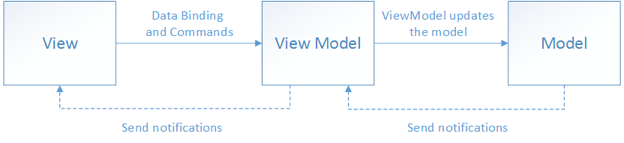
\includegraphics[scale=0.75]{img/mvvm.jpg}
    \caption{Relaciones entre los componentes del patrón MVVM. }
    \label{fig:mvvm}
\end{figure}





El cliente de este proyecto contiene los siguientes paquetes:
\begin{itemize}
    \item \textbf{Componentes}: en este paquete se encuentran los componentes de Angular. Estos componentes se agrupan en otros paquetes según su funcionalidad. Este paquete se corresponde con la Vista y el Modelo de la Vista del patrón MVVM.
    \item \textbf{Servicios}: en este paquete se encuentran los servicios que se comunican con el servidor que es el \textit{backend}. Cada uno de estos servicios manda peticiones HTTP al \textit{backend} para realizar operaciones sobre una entidad del Modelo de Dominio. Este paquete corresponde al Modelo del patrón MVVM.
    \item \textbf{ModelObjects}: en este paquete se encuentran los DTO utilizados para gestionar los datos en el \textit{frontend}. Este paquete también corresponde al Modelo del patrón MVVM.
\end{itemize}

En la Figura \ref{fig:arquitectura-cliente} se muestra la Arquitectura del Cliente.
En las Figuras \ref{fig:componentes-nuevo} a \ref{fig:arq-cli-dto}  se pueden ver los diagramas \textit{Decomposition\&Uses Style} de los paquetes definidos en la Arquitectura del Cliente.




\begin{figure}[H]
    \centering
    \begin{normalsize}
        \import{svg/}{cliente-nuevo.pdf_tex}
    \end{normalsize}
    \caption{Arquitectura del Cliente de la capa de presentación hecho en Angular correspondiente al \textit{frontend}.}
     \label{fig:arquitectura-cliente}
 
 \end{figure}

 \begin{figure}
    \centering
    \begin{normalsize}
        \import{svg/}{componentes-nuevo.pdf_tex}
    \end{normalsize}
    \caption{ \textit{Decomposition\&Uses Style} del paquete \textit{Componentes}.}
     \label{fig:componentes-nuevo}
 
 \end{figure}


 \begin{figure}
    \centering
    \begin{normalsize}
        \import{svg/}{servicios-nuevo.pdf_tex}
    \end{normalsize}
    \caption{ \textit{Decomposition\&Uses Style} del paquete \textit{Servicios}.}
     \label{fig:arq-cli-com}
 
 \end{figure}

 \begin{figure}
    \centering
    \begin{normalsize}
        \import{svg/}{modelobjects-nuevo.pdf_tex}
    \end{normalsize}
    \caption{ \textit{Decomposition\&Uses Style} del paquete \textit{ModelObjects}.}
     \label{fig:arq-cli-dto}
 
 \end{figure}

 


\subsection{Arquitectura del Servidor}

En el servidor que se corresponde con la parte del \textit{backend} desarrollada en NodeJS en la capa lógica se pueden encontrar los siguientes paquetes:
\begin{itemize}
    \item \textbf{Controlador}: en este paquete se encuentra la clase que se encarga de recibir las peticiones HTTP del cliente y de llamar al DAO que realice la operación solicitada.
    \item \textbf{ModelObjects}: en este paquete se encuentran los DTO utilizados para gestionar los datos en el \textit{backend}.
    \item \textbf{DAO}: en este paquete se encuentran los DAO que realizan las operaciones sobre las tablas de la base de datos. 
    \item \textbf{Middleware}: en este paquete se encuentran las clases que se encargarán de procesar las imágenes para almacenarlas en la nube.
\end{itemize}

En la Figura \ref{fig:arquitectura-servidor} se muestra la Arquitectura del Servidor.
En las Figuras \ref{fig:arq-ser-con} a \ref{fig:arq-ser-dao}  se pueden ver los diagramas \textit{Decomposition\&Uses Style} de los paquetes definidos en la Arquitectura del Servidor.

\begin{figure}[H]
    \centering
    \begin{normalsize}
        \import{svg/}{servidor-nuevo.pdf_tex}
    \end{normalsize}
    \caption{Arquitectura del Servidor de la capa lógica hecho en NodeJS correspondiente al \textit{backend}.}
     \label{fig:arquitectura-servidor}
 
 \end{figure}

 \begin{figure}[H]
    \centering
    \begin{normalsize}
        \import{svg/}{arq-ser-con.pdf_tex}
    \end{normalsize}
    \caption{\textit{Decomposition\&Uses Style} del paquete \textit{Controlador}.}
     \label{fig:arq-ser-con}
 
 \end{figure}

 \begin{figure}
    \centering
    \begin{normalsize}
        \import{svg/}{modelobjects-nuevo-serv.pdf_tex}
    \end{normalsize}
    \caption{\textit{Decomposition\&Uses Style} del paquete \textit{ModelObjects}.}
     \label{fig:arq-ser-dto}
 
 \end{figure}

 \begin{figure}[H]
    \centering
    \begin{normalsize}
        \import{svg/}{middleware-serv.pdf_tex}
    \end{normalsize}
    \caption{\textit{Decomposition\&Uses Style} del paquete \textit{Middleware}.}
     \label{fig:arq-ser-dto}
 
 \end{figure}

 \begin{figure}[H]
    \centering
    \begin{normalsize}
        \import{svg/}{arq-ser-dao.pdf_tex}
    \end{normalsize}
    \caption{\textit{Decomposition\&Uses Style} del paquete \textit{DAO}.}
     \label{fig:arq-ser-dao}
 
 \end{figure}




 \section{Patrones de Diseño}

 Para el desarrollo y refinamiento de los subsistemas y componentes software del proyecto se han utilizado diferentes Patrones de Diseño para resolver los problemas encontrados y realizar un sistema más robusto y mejor estructurado. A continuación se enumeran los Patrones de Diseño utilizados. 
 
 \subsection{Observador}
 El patrón Observador \cite{observador} crea un mecanismo en el que se notifica a varios objetos sobre cualquier cambio que sufra un objeto que están observando. Este patrón es uno de los principales utilizados para interfaces gráficas. Los observadores empiezan a observar un determinado objeto suscribiéndose y cuando este objeto cambia se notifica a sus suscriptores los cambios para que realicen las acciones oportunas. Este patrón es el que utiliza para el enlace de datos definido en MVVM, para que los datos entre el Modelo y la Vista estén sincronizados.
 
 En la Figura \ref{fig:patron-observador} se puede ver la estructura del patrón Observador \cite{yania}.
 
 \begin{figure}[H]
     \centering
     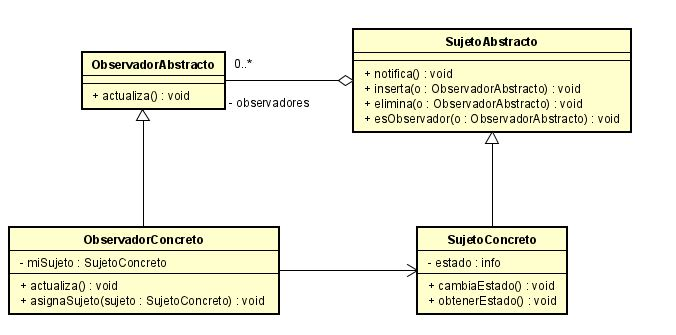
\includegraphics[scale=0.6]{img/observador-nuevo.jpg}
     \caption{Patrón Observador}
     \label{fig:patron-observador}
 \end{figure}
 
 \subsection{DAO/DTO}
 El objetivo del patrón DAO \textit{(Data Access Object)} \cite{DAO}  es independizar la forma de acceder a una fuente de datos, de manera que todo el código que se utilice para acceder a la base de datos se agrupe en una clase DAO. Este patrón proporciona la ventaja de poder modificar la API \textit{ (Application Programming Interface)} de acceso a los datos, de modificar el repositorio de datos, o de facilidades para implementar controles de acceso a los datos como políticas de seguridad. Este patrón permite separar la lógica de negocio de la lógica de datos. 
 
 En este proyecto el patrón DAO se puede ver en el \textit{backend} donde todas las clases DAO se agrupan en el paquete DAO. Cada clase DAO contiene funciones con las diferentes acciones que se pueden realizar sobre una determinada tabla de la base de datos, ya sean de búsqueda, borrado, actualización o creación. 
 
 El patrón DTO \textit{(Data Transfer Object)} \cite{DTO} se utiliza para crear objetos planos que guardan toda la información necesaria que se mostrará en la aplicación con unos atributos que pueden contener información de varias tablas o fuentes. Con el patrón DTO se pueden crear clases especiales para transmitir los datos, almacenando en ellas la información que se desee y teniendo más flexibilidad de manera que se puedan crear estructuras de datos independientes del Modelo de Dominio.
 
 El patrón DTO en Angular permite la creación de interfaces con los atributos deseados para agrupar la información de la manera más organizada posible. De esta manera se facilita la representación de las relaciones entre las tablas de la base de datos mediante la creación de clases DTO con atributos para recoger los valores deseados que representen estas relaciones.  
 
 En este proyecto el patrón DTO se utiliza en Angular en el \textit{frontend} mediante la creación de interfaces, cada una correspondiendo con una clase del Modelo de Dominio. Cada clase DTO tiene los atributos de la clase del Modelo de Dominio y otros atributos que guarden otra información necesaria de esa clase debido a las relaciones que tiene con otras tablas. En NodeJS en el \textit{backend} también se utiliza este patrón de la misma manera.
 
 En la Figura \ref{fig:patrondaodto} se puede ver la combinación de los patrones DAO y DTO \cite{yania}.
 
 \begin{figure}[H]
     \centering
     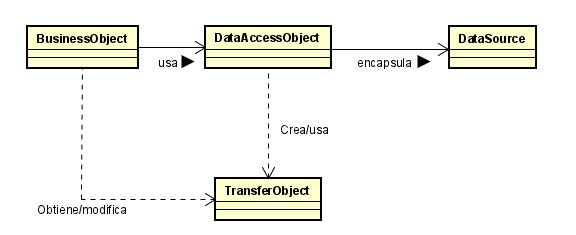
\includegraphics[scale=0.7]{img/dao-nuevo.jpg}
     \caption{Patrón DAO/DTO}
     \label{fig:patrondaodto}
 \end{figure}
 
 \subsection{\textit{Singleton}}
 El patrón \textit{Singleton} \cite{Singleton} se encarga de que solo exista una única instancia de una determinada clase, de manera que restringe la libre creación mediante diferentes técnicas. Por otro lado, establece un método para obtener esa instancia. De esta manera, solo existe una única instancia de la clase en toda la aplicación y es accesible de manera global.
 
 Angular proporciona los \textit{Singleton Services} que son servicios que tienen una sola instancia en toda la aplicación, de esta manera se tiene el control sobre cuándo y como se accede a este servicio \cite{Singleton-Services}. 
 
 Este patrón es utilizado en los servicios de Angular que realizan las peticiones al \textit{backend} de manera que solo exista una instancia de cada servicio.
 
 En la Figura \ref{fig:singleton} se puede ver la estructura del patrón \textit{Singleton} \cite{yania}.
 
 \begin{figure}
     \centering
     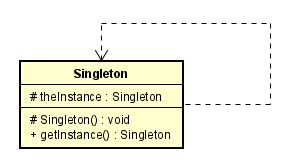
\includegraphics[scale=0.7]{img/singleton-nuevo.jpg}
     \caption{Patrón Singleton}
     \label{fig:singleton}
 \end{figure}





\section{Arquitectura Física del Sistema}
El Diseño de Despliegue \cite{diagrama-despliegue} se realiza para definir los dispositivos del sistema, sus enlaces de comunicación entre ellos y cómo se distribuyen los archivos del sistema entre ellos. Muestra la arquitectura en ejecución del sistema incluyendo su \textit{hardware}, \textit{software} y \textit{middleware}. Para realizar el Diseño de Despliegue se definirá un Diagrama de Despliegue que contendrá los dispositivos dentro del sistema junto a los elementos \textit{software} dentro de ellos y las relaciones entre estos dispositivos. 

En la Figura \ref{fig:diagrama-despliegue} se muestra el Diagrama de Despliegue de la aplicación Web.

\begin{figure}
    \centering
    \begin{normalsize}
        \import{svg/}{despliegue-escalado.pdf_tex}
    \end{normalsize}
    \caption{Diagrama de Despliegue}
     \label{fig:diagrama-despliegue}
 
 \end{figure}



 \section{Diseño de la Base de Datos}
El Diseño de la Base de Datos \cite{diseno-base} es el proceso para definir la estructura adecuada de la base de datos que almacenará toda la información de la aplicación. Para ello se deben definir las diferentes tablas que se almacenarán en la base de datos, sus atributos junto a su tipo y las relaciones entre las diferentes tablas mediante las claves primarias y foráneas. Para el Diseño de la Base de Datos se va a utilizar un Diagrama de la Base de Datos que contendrá las tablas de la base de datos con sus atributos y su tipo y las relaciones entre ellas. Para diseñar la base de datos se ha utilizado como diagrama conceptual el Diagrama de Clases del Modelo de Dominio que se encuentra en la sección \ref{sec:clases} a partir del cuál se han sacado las tablas de la base de datos.

En la Figura \ref{fig:diagrama-basedatos} se muestra el Diseño de la Base de Datos mediante su Diseño
Lógico, para ello se utiliza una representación basada en UML con estereotipos. 
Los estereotipos <<PK>> y <<FK>> representan las claves primarias y foráneas. El estereotipo <<table>> sirve para representar una tabla en el esquema relacional. El estereotipo <<entity>> está en las tablas que representan un elemento del Dominio.

\begin{figure}
    \centering
    \begin{normalsize}
        \import{svg/}{basedatos-escalado.pdf_tex}
    \end{normalsize}
    \caption{Diseño Lógico de la Base de Datos}
     \label{fig:diagrama-basedatos}
 
 \end{figure}



\section{Diseño de la Interfaz Gráfica}
El \textit{frontend} \cite{frontend} de un sitio Web son todas las tecnologías de diseño y desarrollo Web que se visualizan en un navegador, es decir, la parte visible para los usuarios y tienen como fin interactuar con el Usuario que utilice el sitio Web. Determinará en gran medida el número de clientes de la aplicación.

La interfaz gráfica es fundamental para que los usuarios puedan navegar por la página Web, para ello el \textit{frontend}  se conecta con el \textit{backend} para acceder a todos los contenidos que estén almacenados en la base de datos. Si la interfaz de una aplicación Web no está bien construida, el cliente podría abandonar el sitio Web porque no entiende cómo funciona.  

Por lo tanto, los objetivos que debe cumplir el \textit{frontend} son implementar los elementos visuales del sitio Web de manera que se facilite la interacción con el Usuario, mandar los datos recogidos en la interfaz al \textit{backend} de manera adecuada para que pueda almacenarlos y saber interpretar los datos que envíe el \textit{backend} para mostrárselos de manera adecuada al Usuario.



Otro aspecto importante, es cómo funciona la interfaz en los dispositivos móviles, ya que el uso de \textit{smartphones} y \textit{tablets} está completamente implementado en la sociedad actual. Por lo tanto para aumentar el número de usuarios es fundamental que la aplicación Web funcione desde cualquier dispositivo sea cual sea su tamaño de pantalla \cite{frontend-importancia}.

La experiencia de usuario \cite{experiencia-usuario} hace referencia a como se siente el Usuario al interactuar con el sistema. Aspectos sobre esto son la facilidad de uso, la utilidad, el valor percibido y la eficiencia a la hora de realizar una tarea. Una buena experiencia de usuario es fundamental para atraer usuarios. La experiencia del usuario ha tomado relevancia debido a las siguientes razones:

\begin{itemize}
    \item \textbf{La complejidad de las páginas Web ha aumentado.} Actualmente las aplicaciones Web tienen muchas funcionalidades y contenidos. 
    \item \textbf{Dispositivos diferentes.} Los usuarios acceden a las aplicaciones Web desde multitud de dispositivos diferentes.  
    \item \textbf{Cada vez se valora más la accesibilidad.} Es importante que la aplicación Web se adapte a todo tipo de usuarios, tanto como los que tienen problemas visuales como los que tienen una conexión lenta o un dispositivo antiguo.  
    \item \textbf{Exigencias de los usuarios.} La aplicación Web tiene que crear un producto único y de calidad, que haga que la experiencia de usuario sea agradable.  
\end{itemize}


Los bocetos aquí creados sirven como ideas previas al desarrollo final de cada vista de la aplicación, por lo tanto la interfaz final desarrollada puede variar ligeramente respecto a estos bocetos. Por otro lado, estos bocetos son diseños simplificados de las interfaces que compondrán la aplicación Web, que principalmente se utilizarán como referencia para ver la estructura y organización de los elementos que compondrán cada pantalla de la aplicación. Por ello, los detalles más específicos como los colores no se han incluido en muchos de estos bocetos. 

Se ha creado un componente de Angular por cada interfaz que se pueda acceder en la aplicación Web. También se han definido componentes para representar a las entidades del Modelo de Dominio que se muestran en la aplicación, de manera que cada instancia de una entidad se muestra mediante una carta donde se muestra la información relevante.  

En las Figuras \ref{fig:carta-receta} a \ref{fig:carta-alimento-receta} se muestran los bocetos de las cartas que se utilizarán para resumir los datos principales de cada elemento que se mostrará en la aplicación.




\begin{figure}[H]
    \centering
    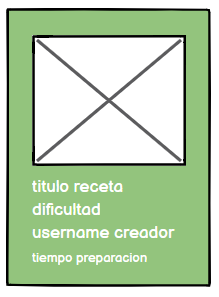
\includegraphics{img/carta-receta.jpg}
    \caption{Boceto de la carta de una receta}
    \label{fig:carta-receta}
\end{figure}




\begin{figure}[H]
    \centering
    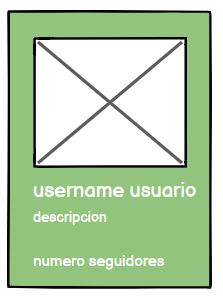
\includegraphics{img/carta-usuario.jpg}
    \caption{Boceto de la carta de un Usuario}
    \label{fig:carta-usuario}
\end{figure}




\begin{figure}[H]
    \centering
    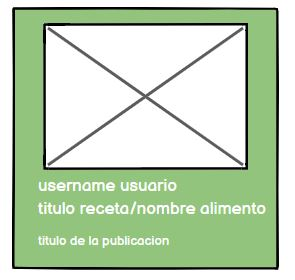
\includegraphics{img/carta-publicacion.jpg}
    \caption{Boceto de la carta de una publicación}
    \label{fig:carta-publicacion}
\end{figure}




\begin{figure}[H]
    \centering
    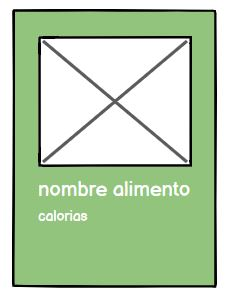
\includegraphics{img/carta-alimento.jpg}
    \caption{Boceto de la carta de un alimento}
    \label{fig:carta-alimento}
\end{figure}



\begin{figure}[H]
    \centering
    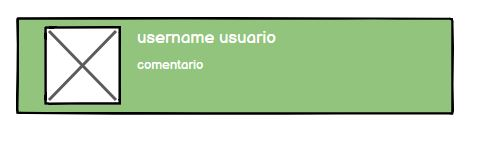
\includegraphics{img/carta-comentario.jpg}
    \caption{Boceto de la carta de un comentario}
    \label{fig:carta-comentario}
\end{figure}




\begin{figure}[H]
    \centering
    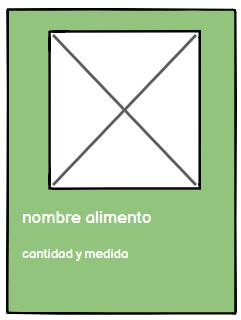
\includegraphics{img/carta-alimento-receta.jpg}
    \caption{Boceto de la carta de un alimento incluido en una receta}
    \label{fig:carta-alimento-receta}
\end{figure}






En las Figuras \ref{fig:descripcion-aplicacionPrimera} a \ref{fig:vista-admin} se muestran los bocetos de las interfaces que permitirán la navegación por la aplicación y que utilizarán esas cartas. 



\begin{figure}[H]
    \centering
    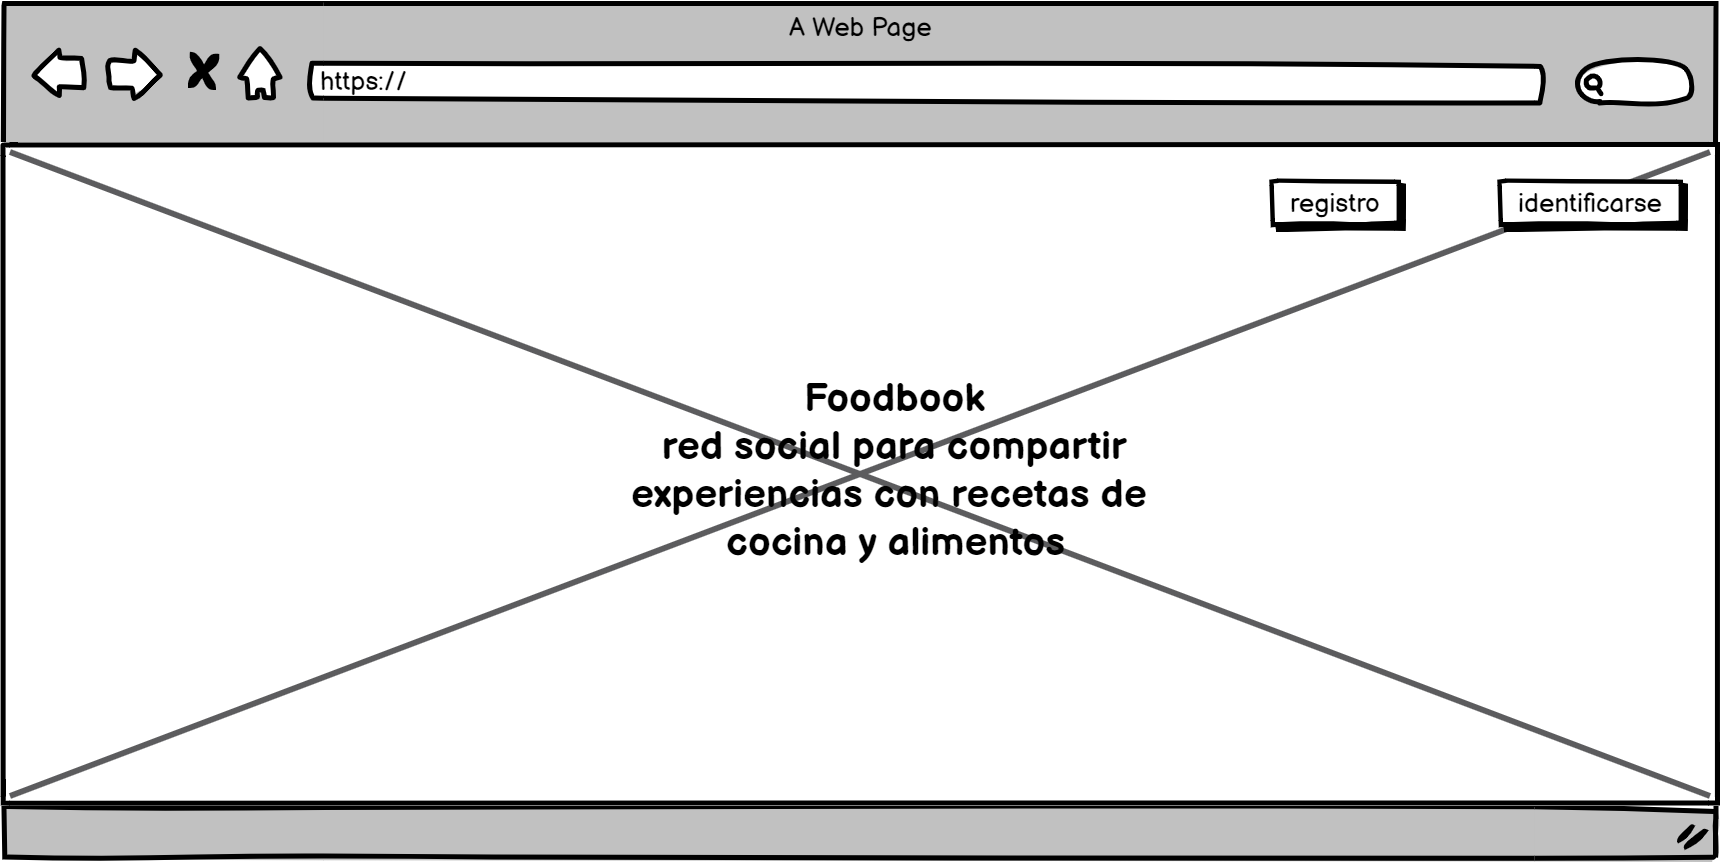
\includegraphics[scale=0.20]{img/descripcion-aplicacion1.jpg}
    \caption{Parte superior del boceto de la interfaz de descripción de la aplicación.}
    \label{fig:descripcion-aplicacionPrimera}
\end{figure}


\begin{figure}[H]
    \centering
    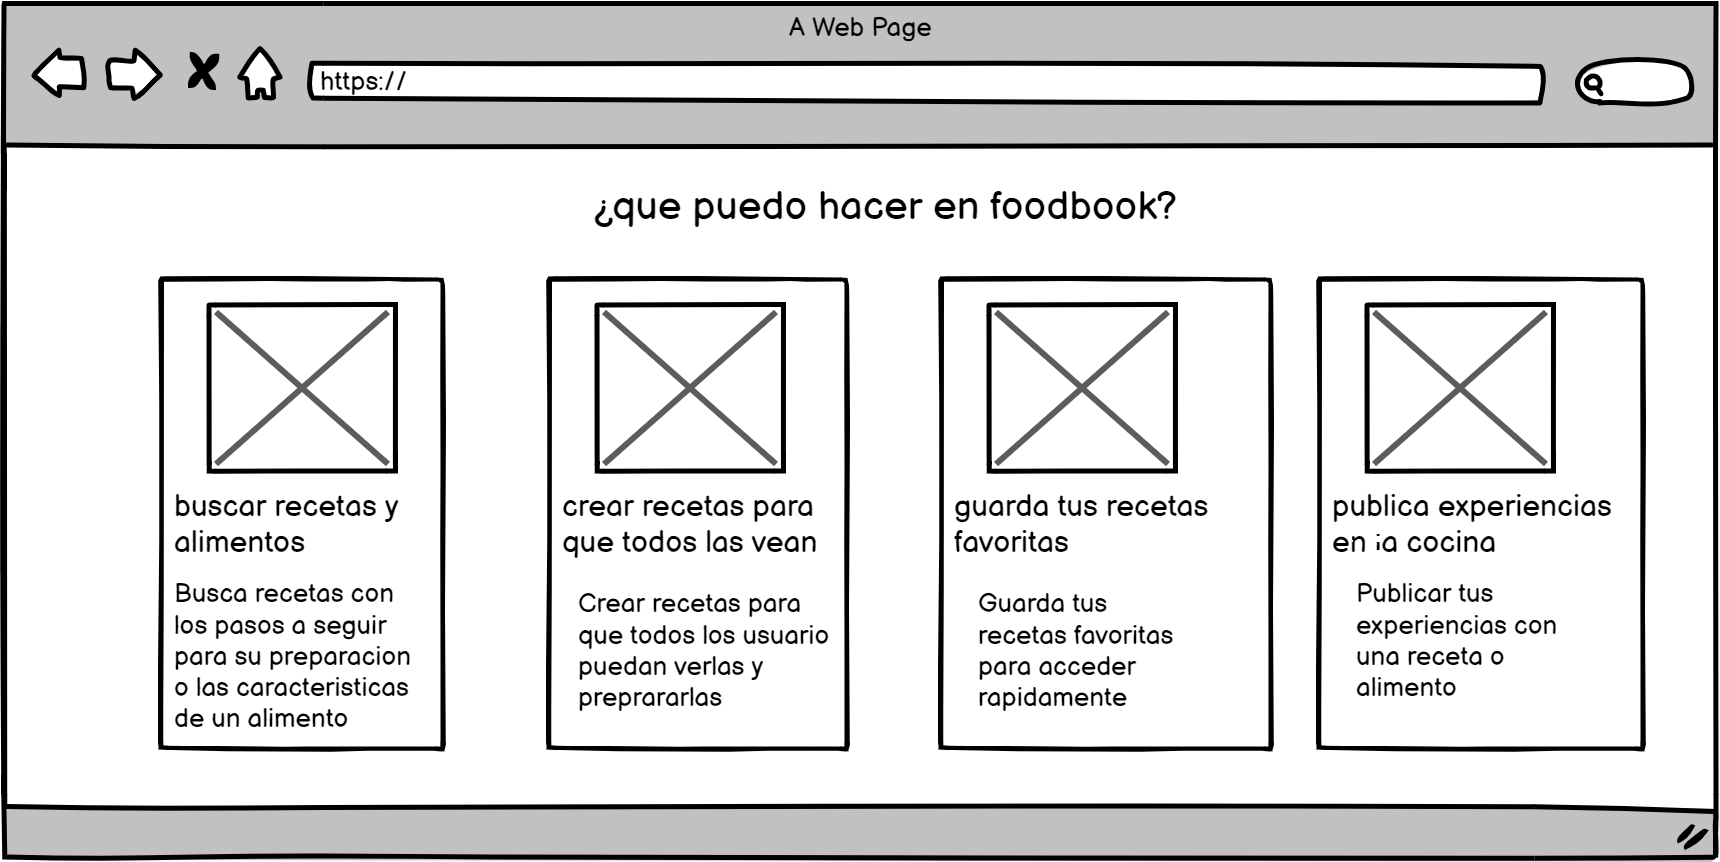
\includegraphics[scale=0.20]{img/descripcion-aplicacion2.jpg}
    \caption{Parte inferior del boceto de la interfaz de descripción de la aplicación.}
    \label{fig:descripcion-aplicacion2}
\end{figure}



 
    
\begin{figure}[H]
    \centering
    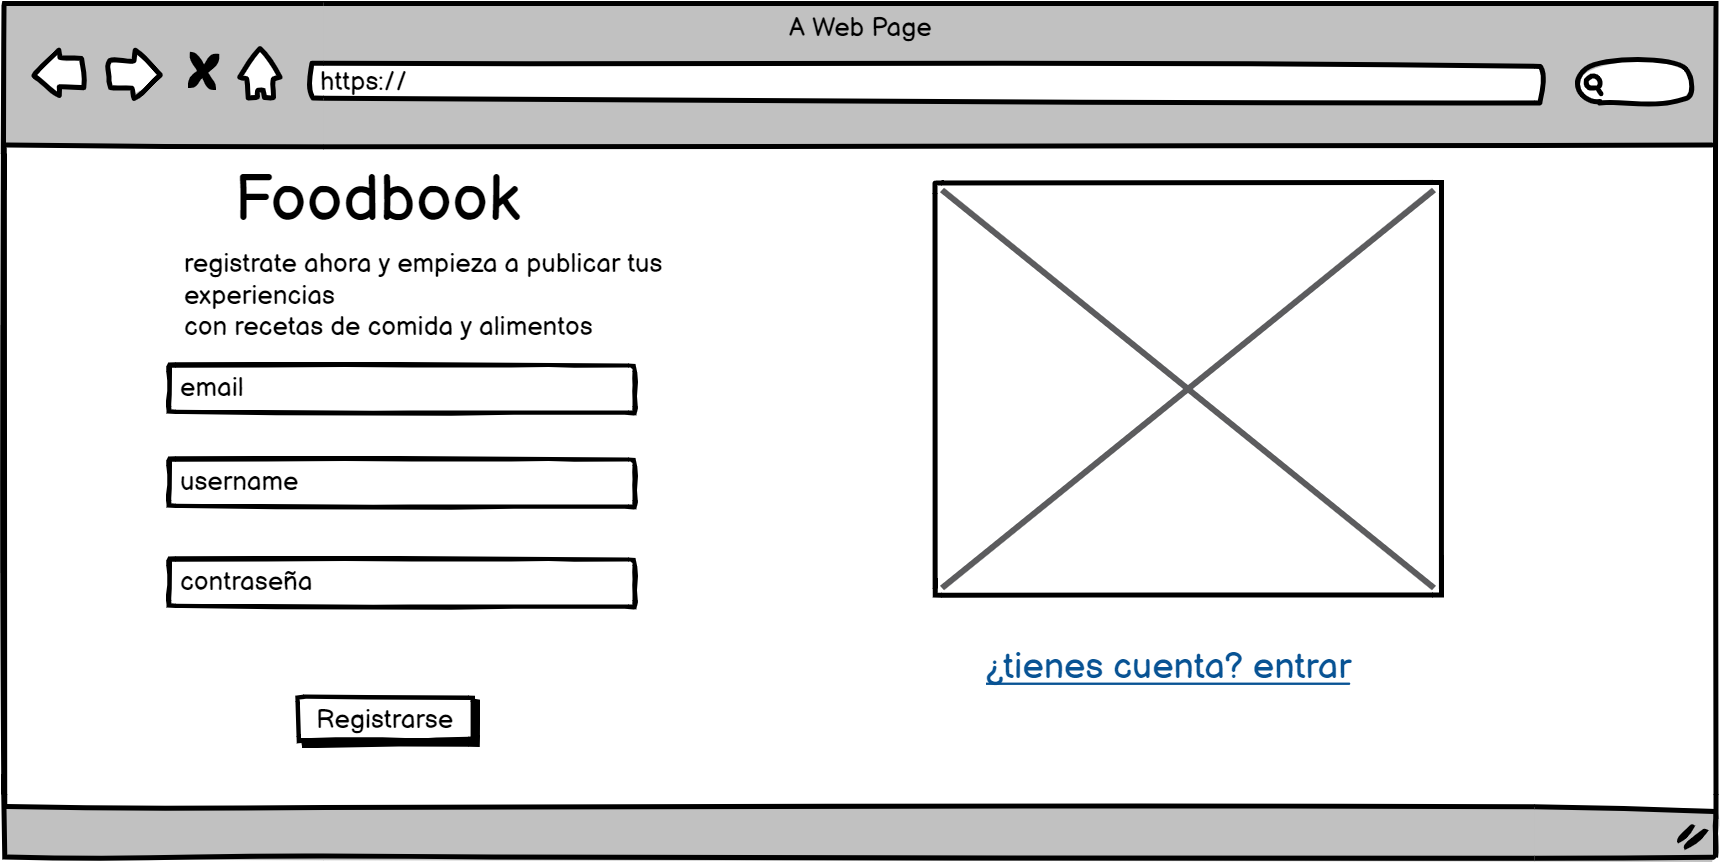
\includegraphics[scale=0.20]{img/registro-usuario.jpg}
    \caption{Boceto de la interfaz de registro de un Usuario.}
    \label{fig:registro-usuario}
\end{figure}
 

\begin{figure}[H]
    \centering
    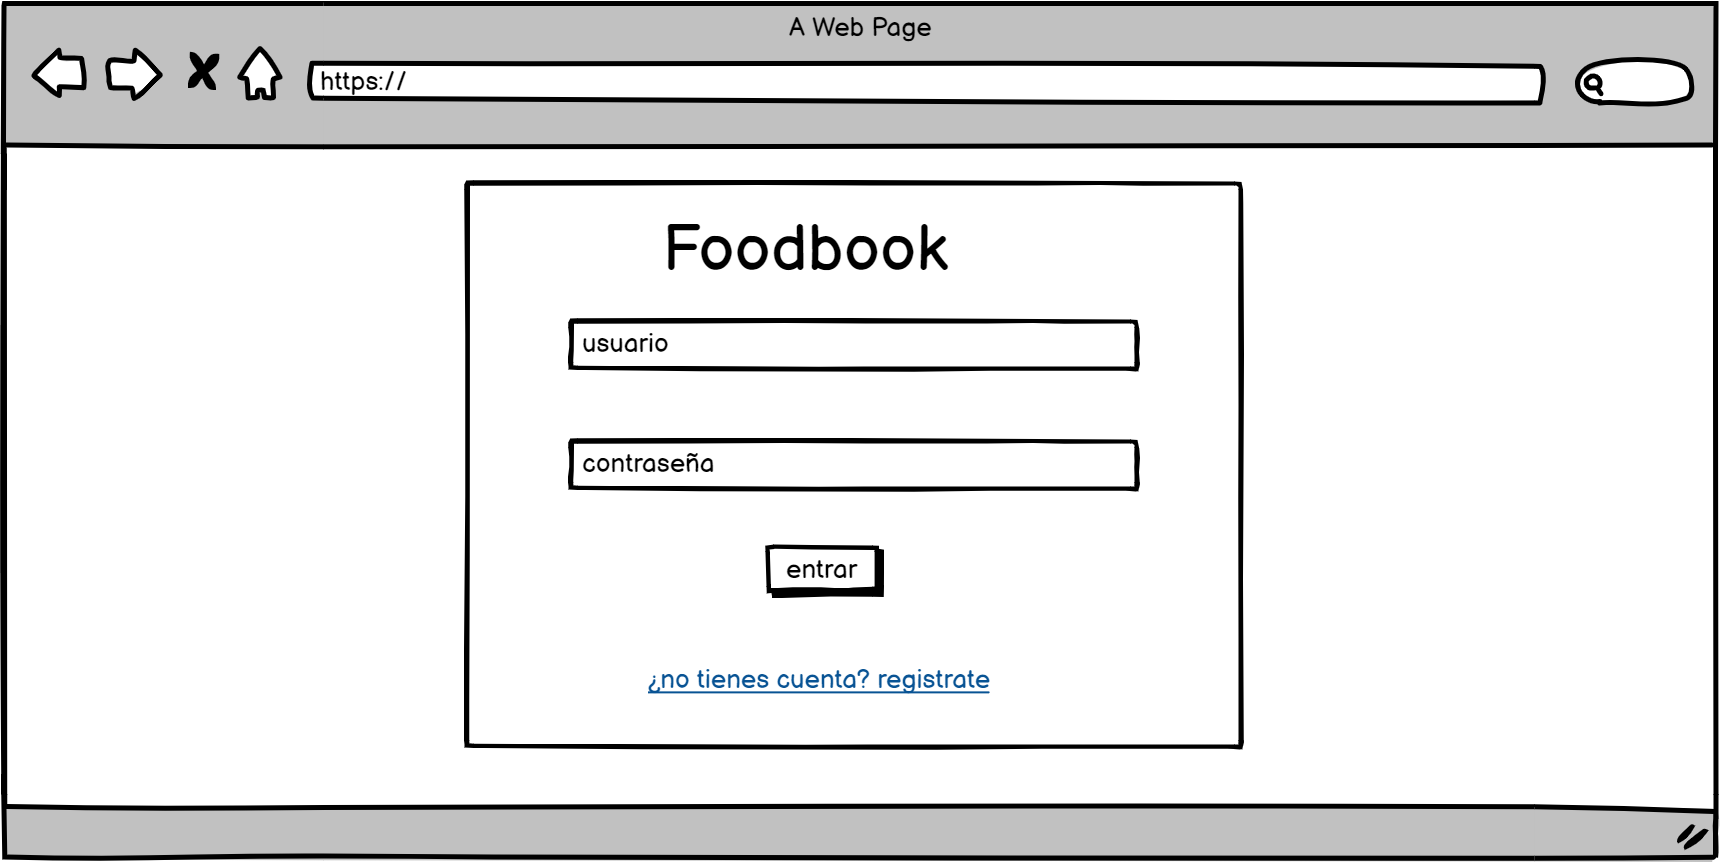
\includegraphics[scale=0.20]{img/identificacion-usuario.jpg}
    \caption{Boceto de la interfaz de identificación de un Usuario.}
    \label{fig:identificacion-usuario}
\end{figure}

   
    \begin{figure}[H]
    \centering
    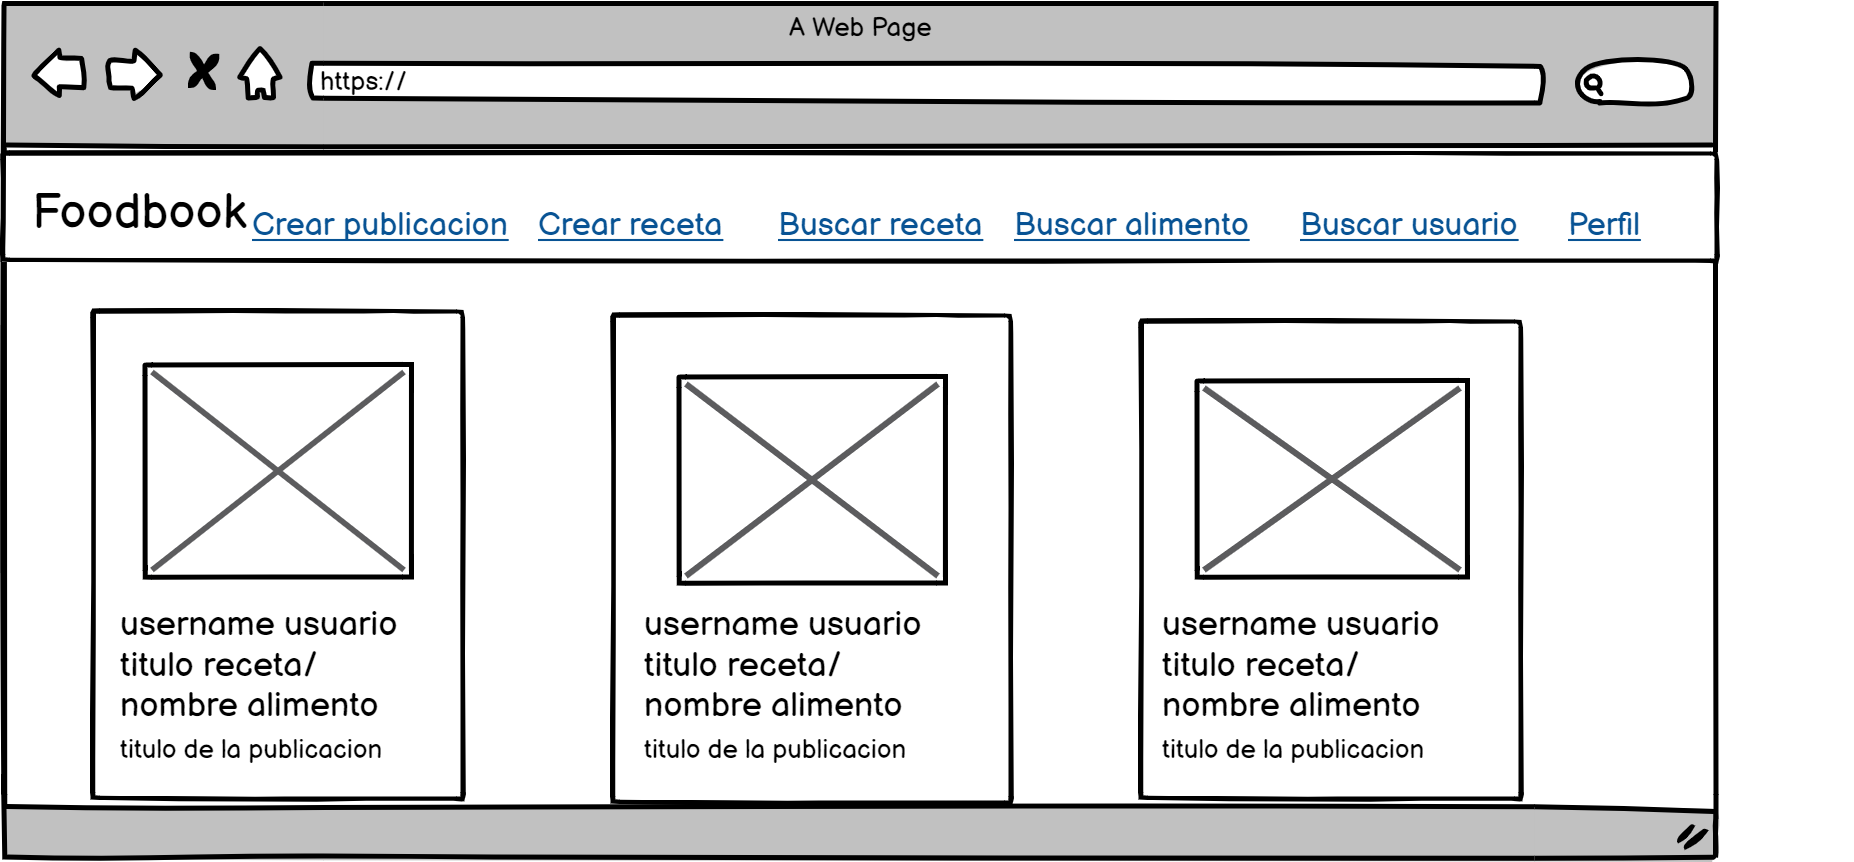
\includegraphics[scale=0.20]{img/muro-publicaciones.jpg}
    \caption{Boceto de la interfaz de muro de publicaciones.}
    \label{fig:muro-publicaciones}
\end{figure}
    
  
    \begin{figure}[H]
    \centering
    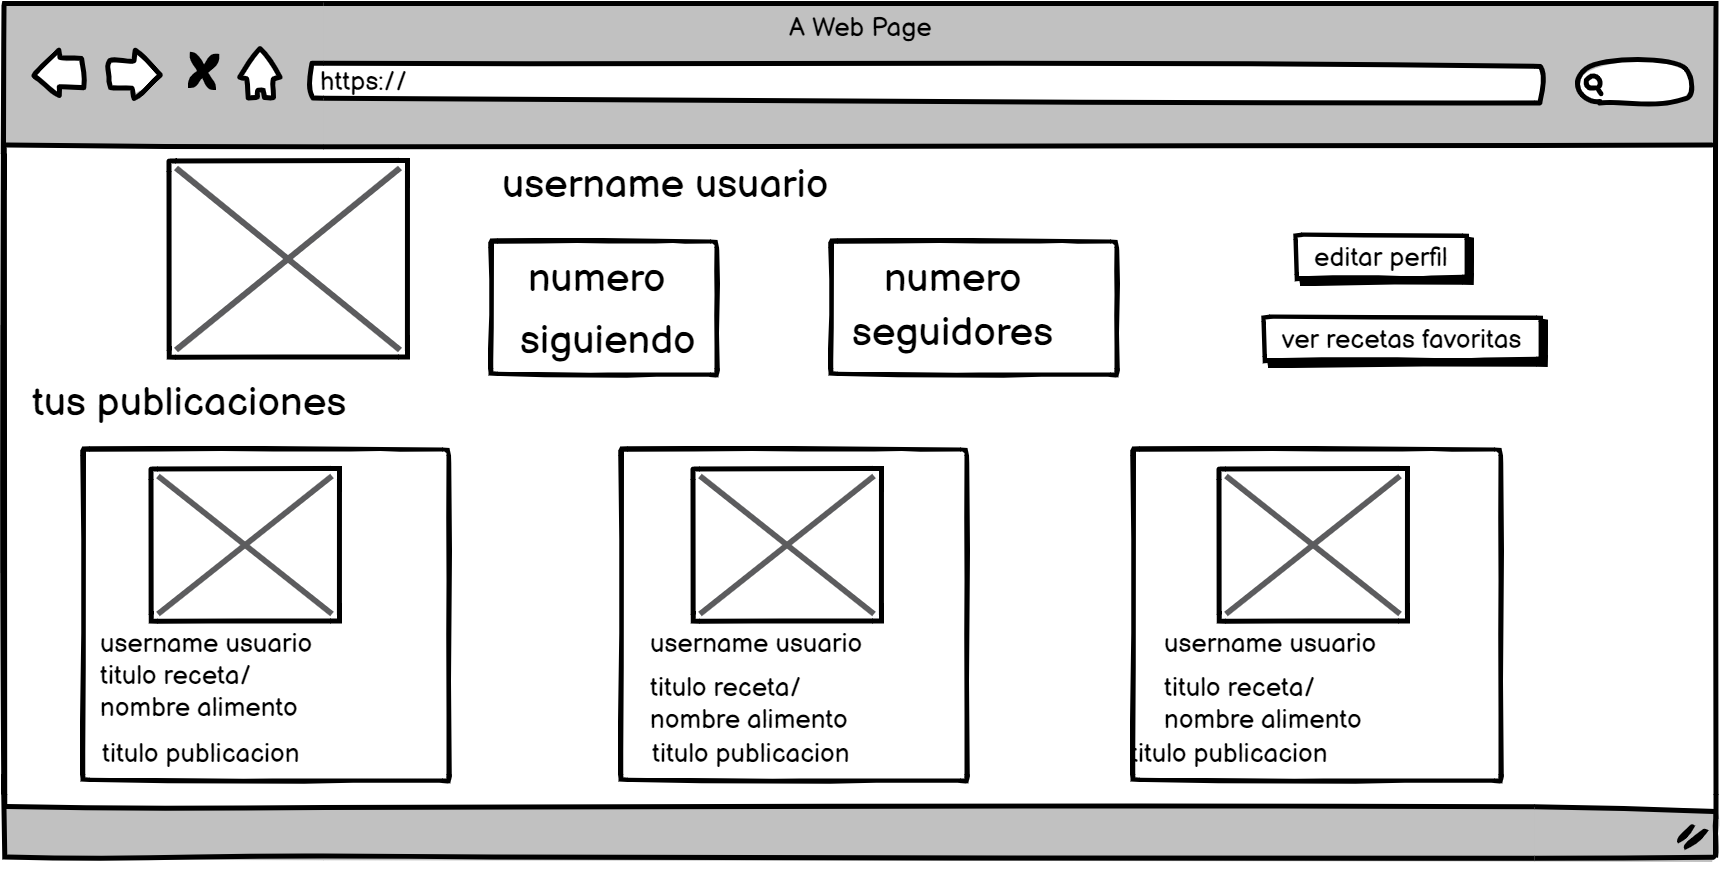
\includegraphics[scale=0.20]{img/perfil-usuario.jpg}
    \caption{Boceto de la interfaz de perfil del Usuario.}
    \label{fig:perfil-usuario}
\end{figure}
    
   

     \begin{figure}[H]
    \centering
    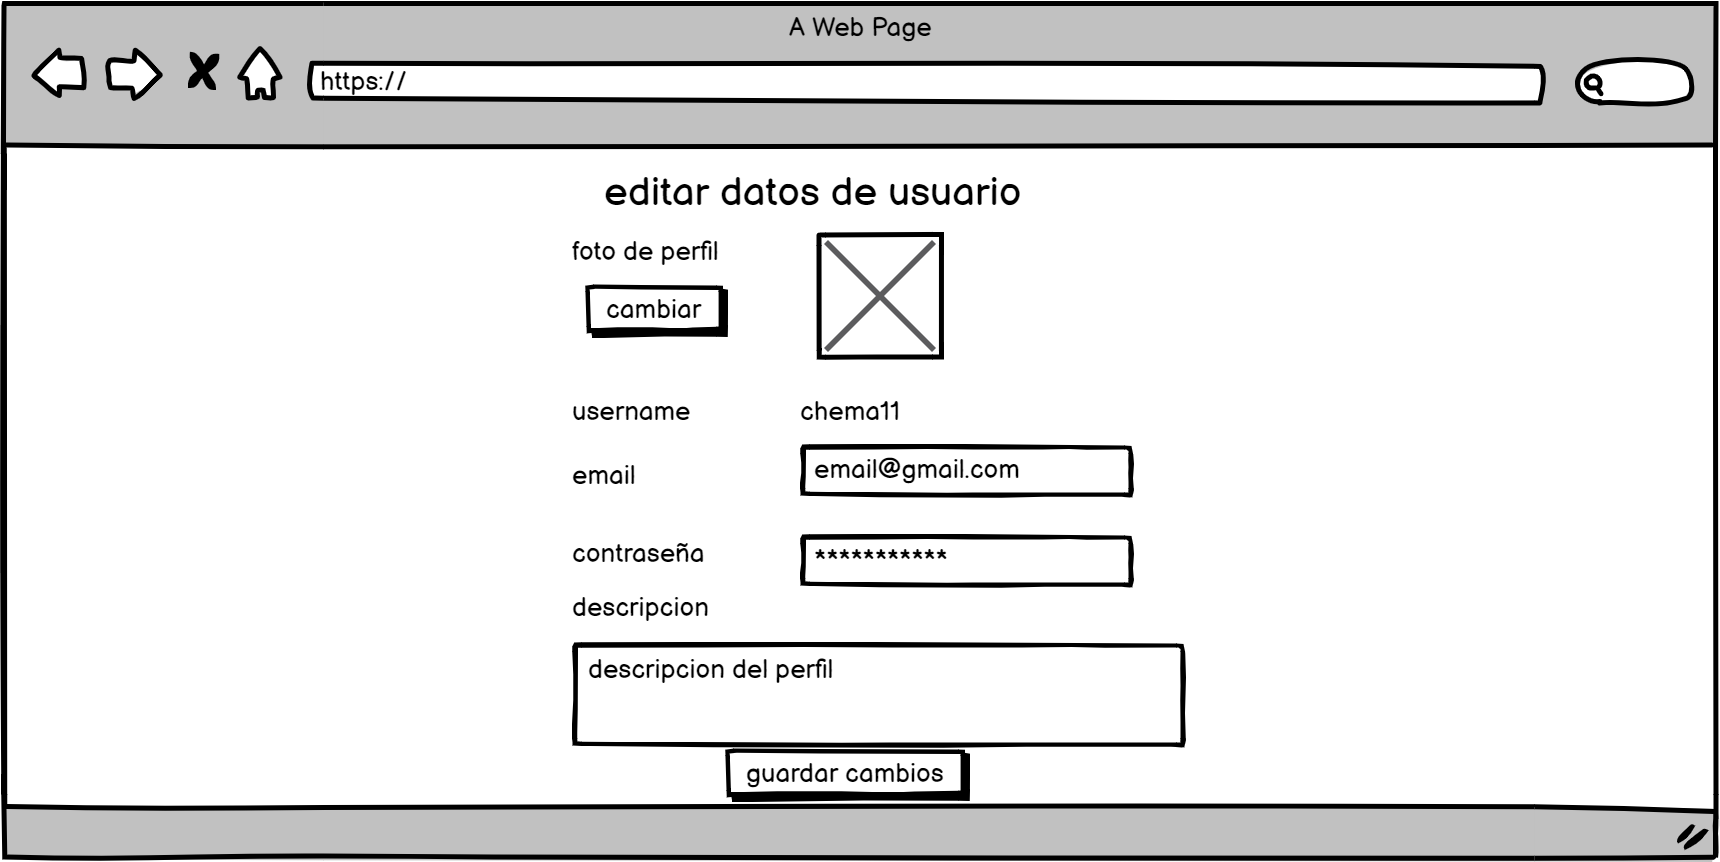
\includegraphics[scale=0.20]{img/editar-usuario.jpg}
    \caption{Boceto de la interfaz de editar perfil del Usuario.}
    \label{fig:editar-usuario}
\end{figure}
    
 

     \begin{figure}[H]
    \centering
    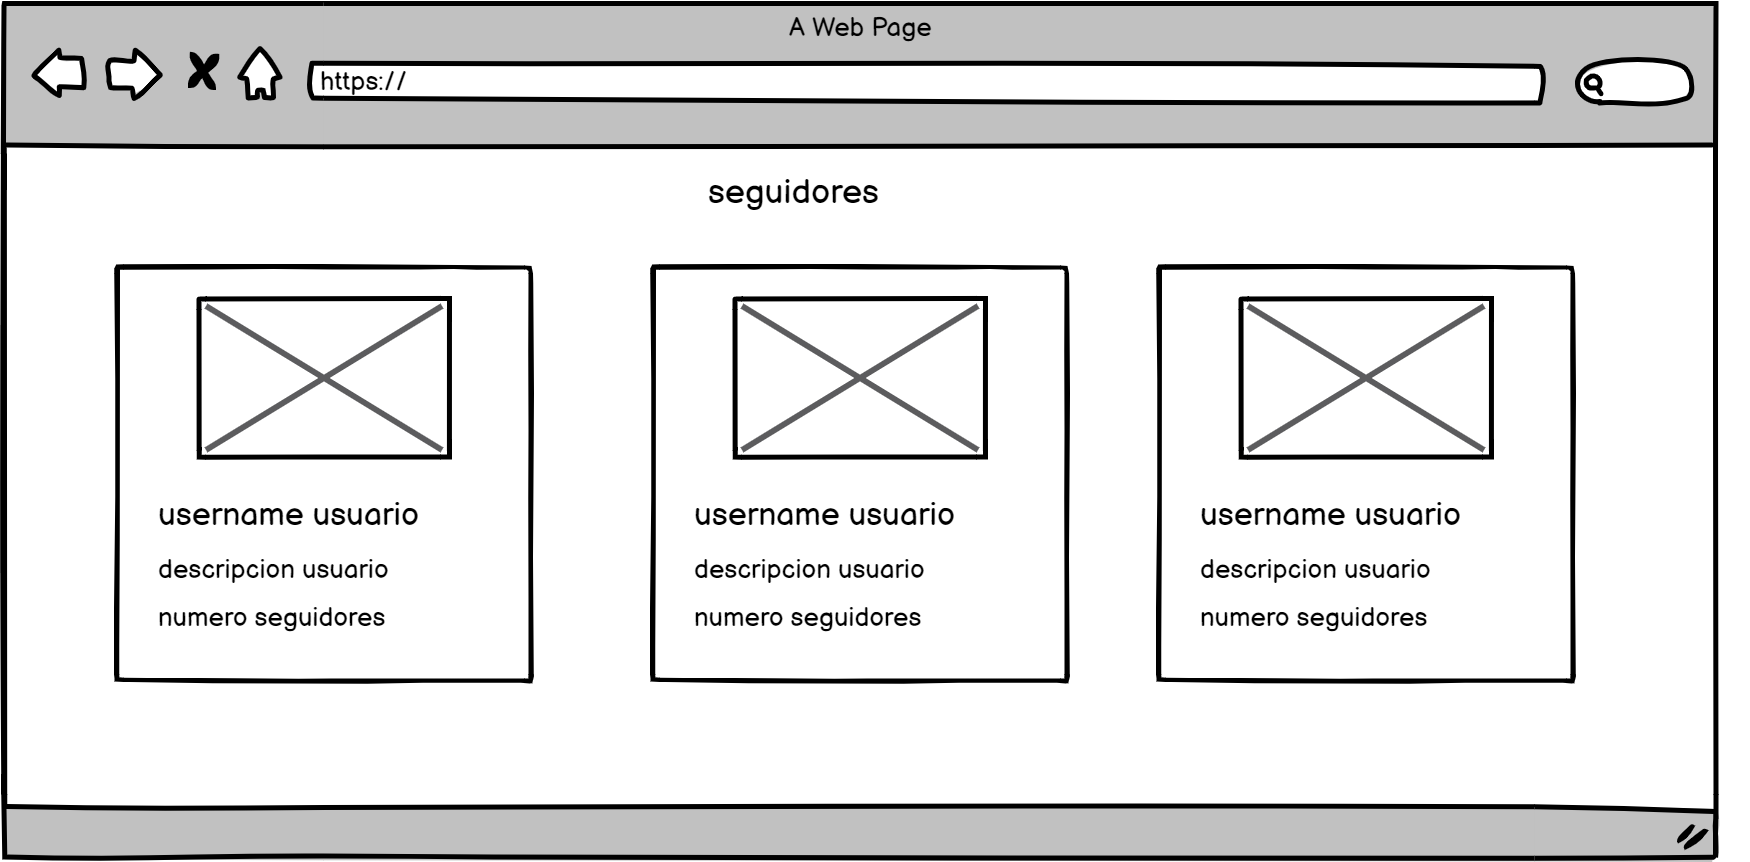
\includegraphics[scale=0.20]{img/seguidores-usuario.jpg}
    \caption{Boceto de la interfaz de seguidores del Usuario.}
    \label{fig:seguidores-usuario}
\end{figure}
    
  

     \begin{figure}[H]
    \centering
    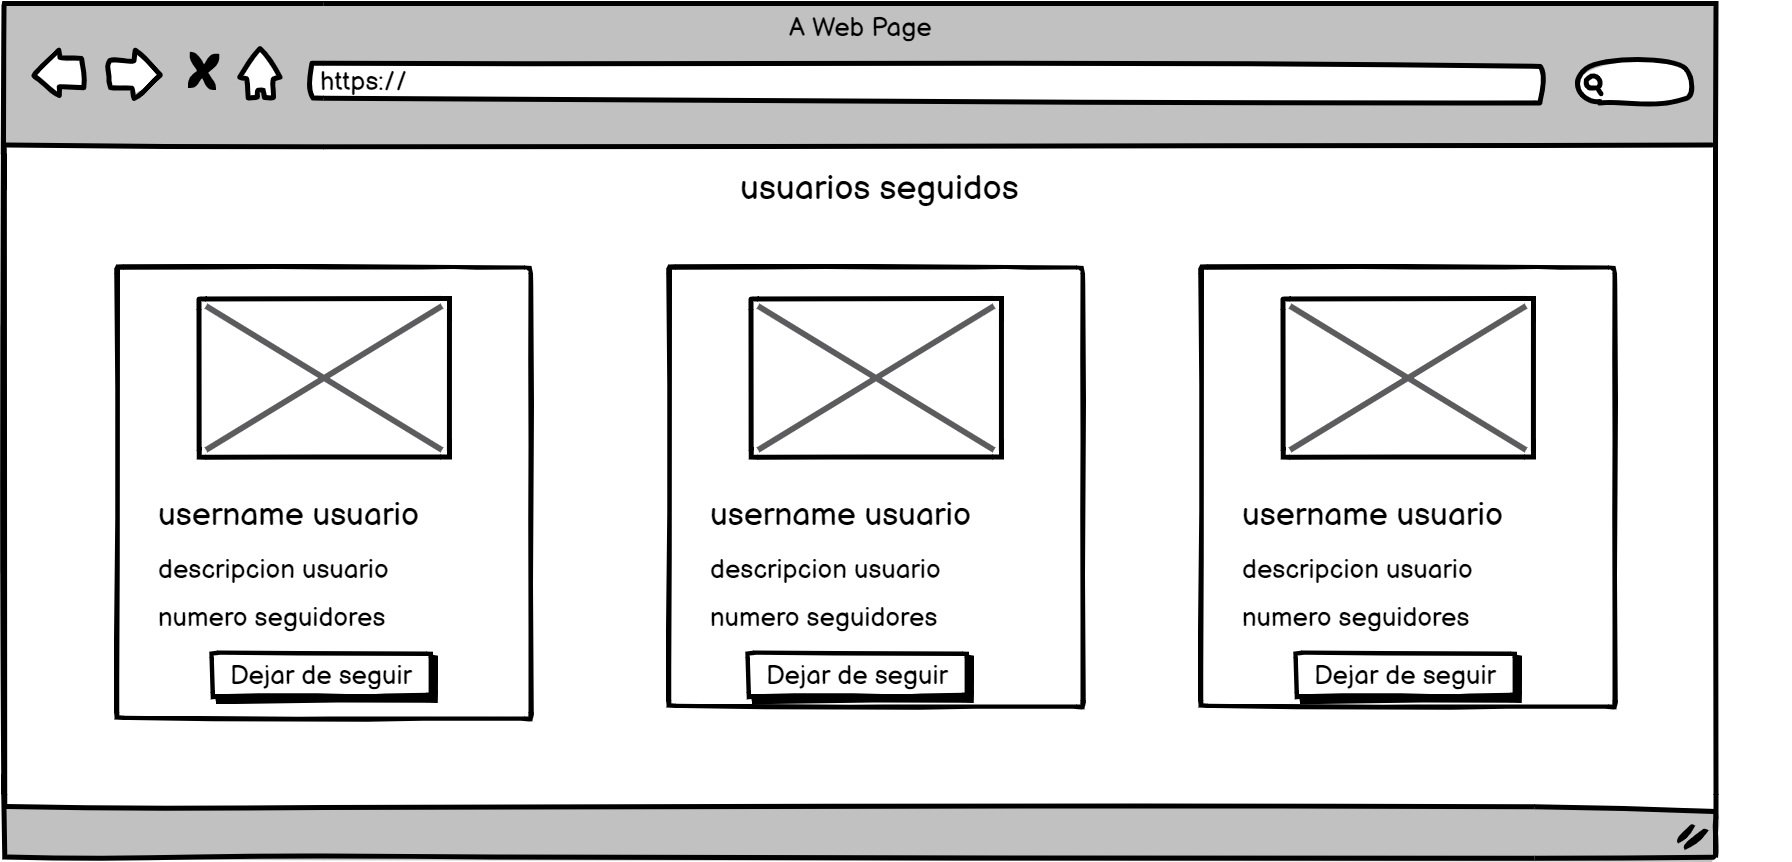
\includegraphics[scale=0.20]{img/seguidos-usuario.jpg}
    \caption{Boceto de la interfaz de seguidos del Usuario.}
    \label{fig:seguidos-usuario}
\end{figure}
    
   

      \begin{figure}[H]
    \centering
    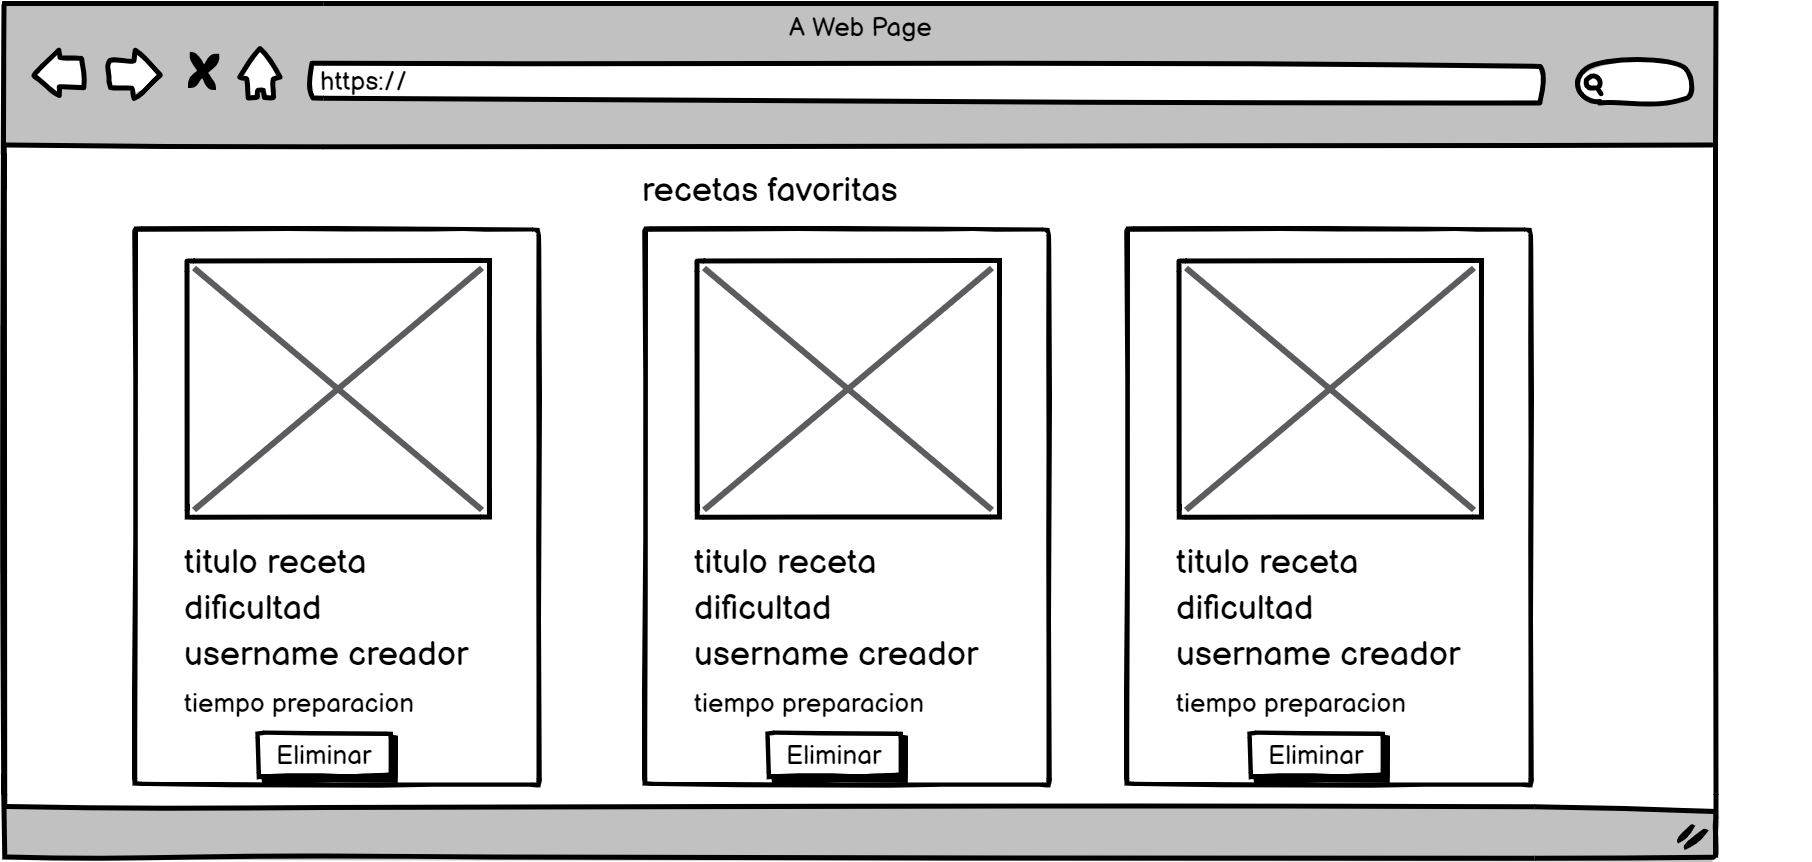
\includegraphics[scale=0.20]{img/favoritas-recetas.jpg}
    \caption{Boceto de la interfaz de recetas favoritas.}
    \label{fig:favoritas-recetas}
\end{figure}
    
  

     \begin{figure}[H]
    \centering
    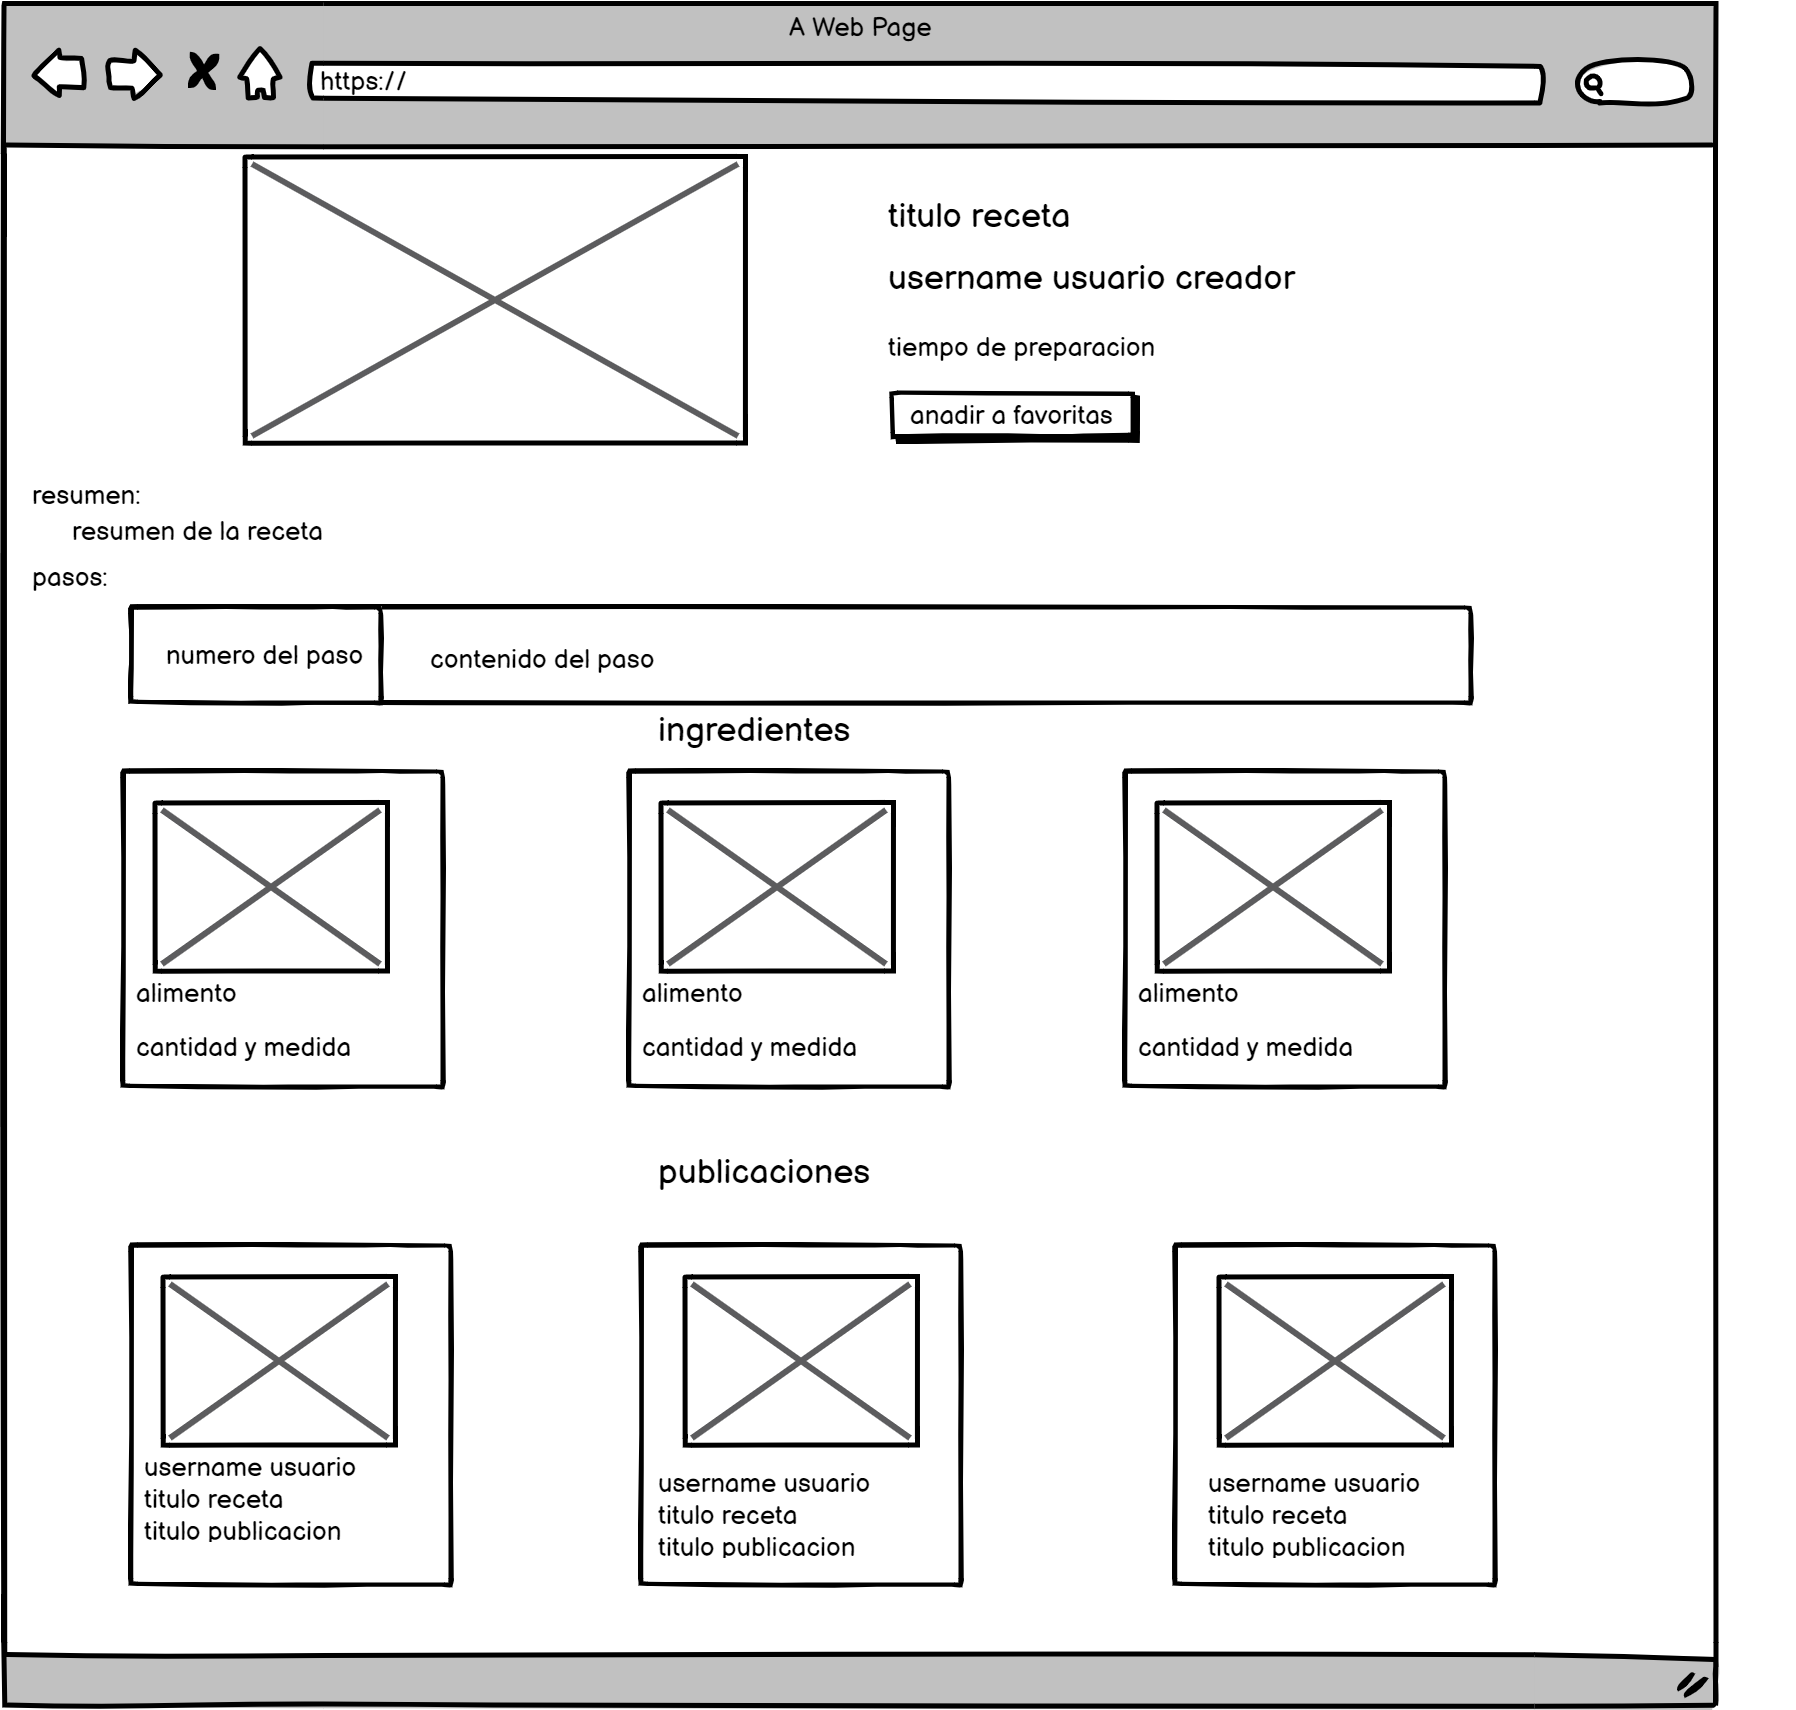
\includegraphics[scale=0.20]{img/detalle-receta.jpg}
    \caption{Boceto de la interfaz de detalles de la receta.}
    \label{fig:detalle-receta}
\end{figure}
    
   

     \begin{figure}[H]
    \centering
    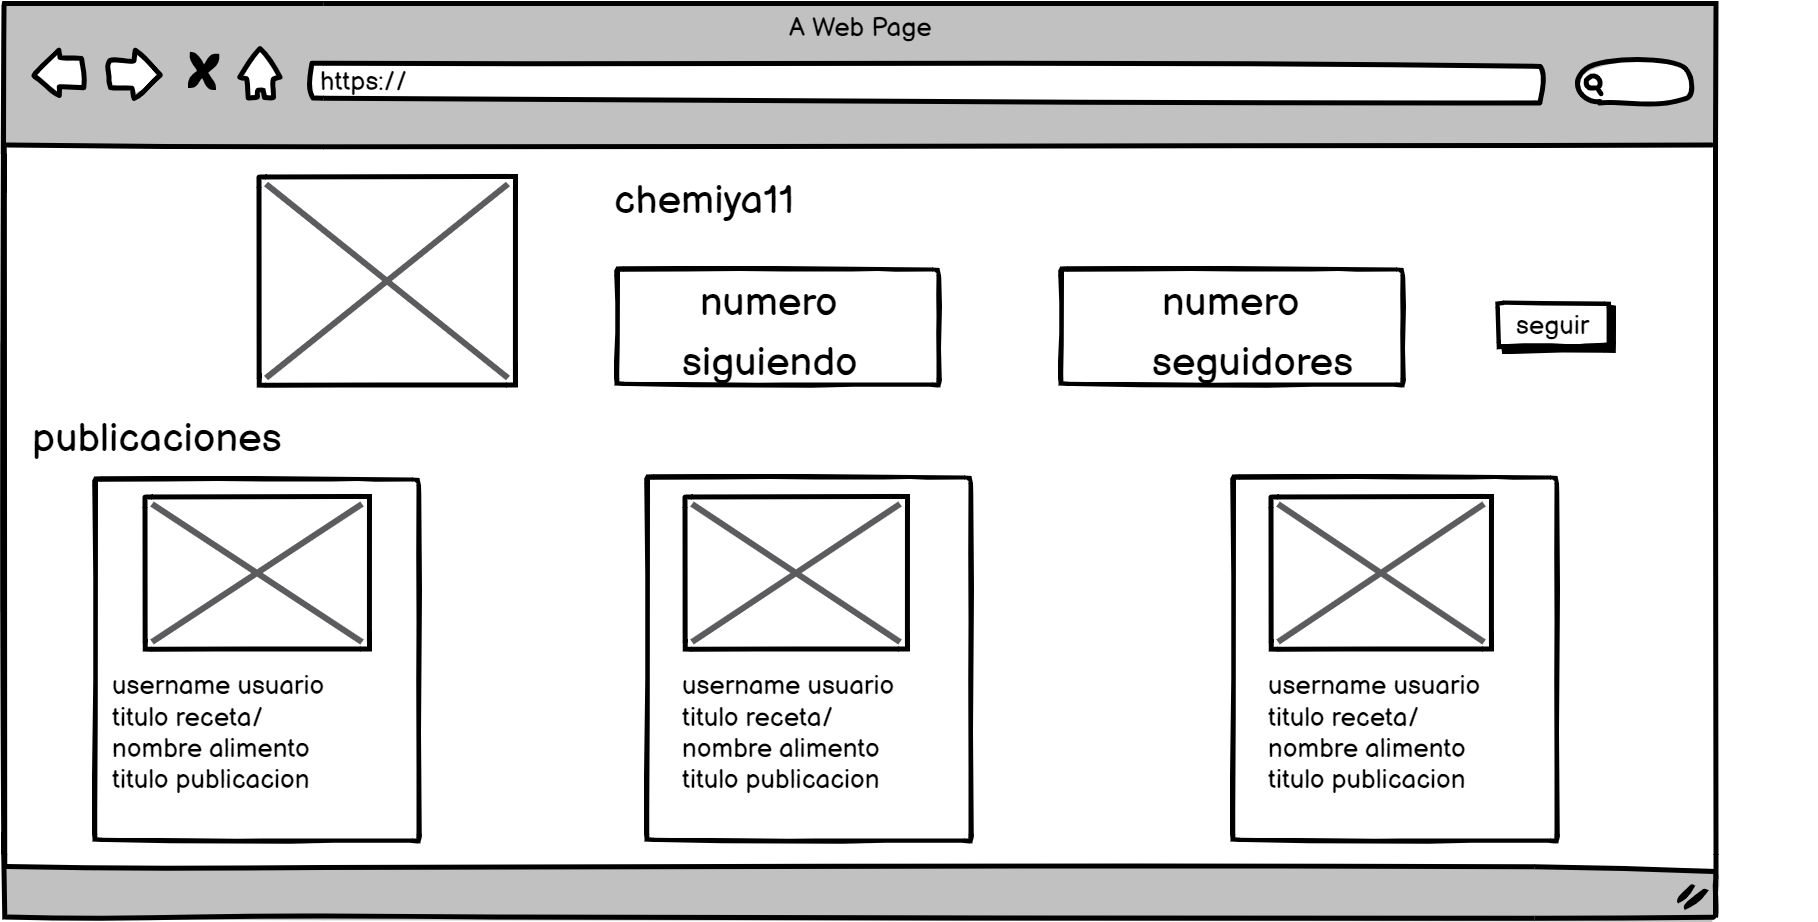
\includegraphics[scale=0.20]{img/detalle-usuario.jpg}
    \caption{Boceto de la interfaz de detalles del Usuario.}
    \label{fig:detalle-usuario}
\end{figure}
    
   

     \begin{figure}[H]
    \centering
    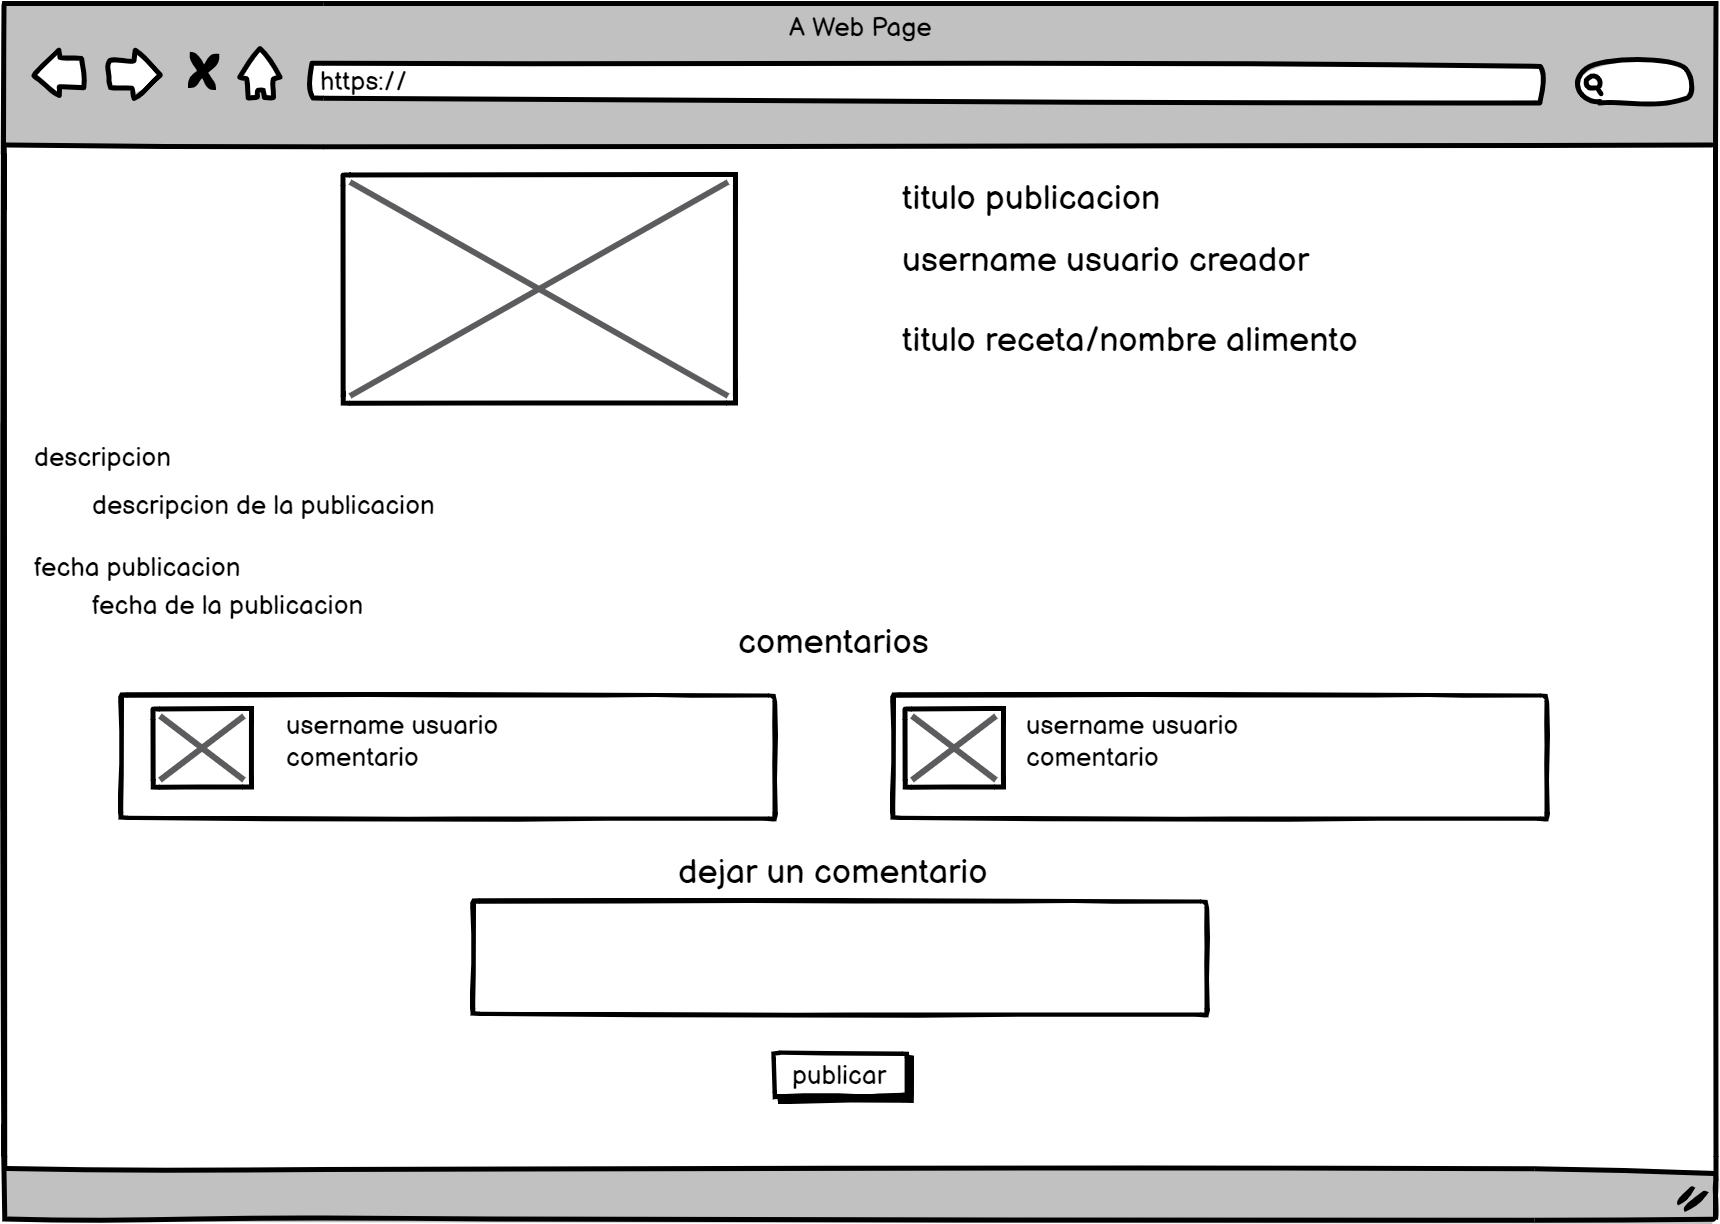
\includegraphics[scale=0.20]{img/detalle-publicacion.jpg}
    \caption{Boceto de la interfaz de detalles de la publicación.}
    \label{fig:detalle-publicacion}
\end{figure}
    
     

     \begin{figure}[H]
    \centering
    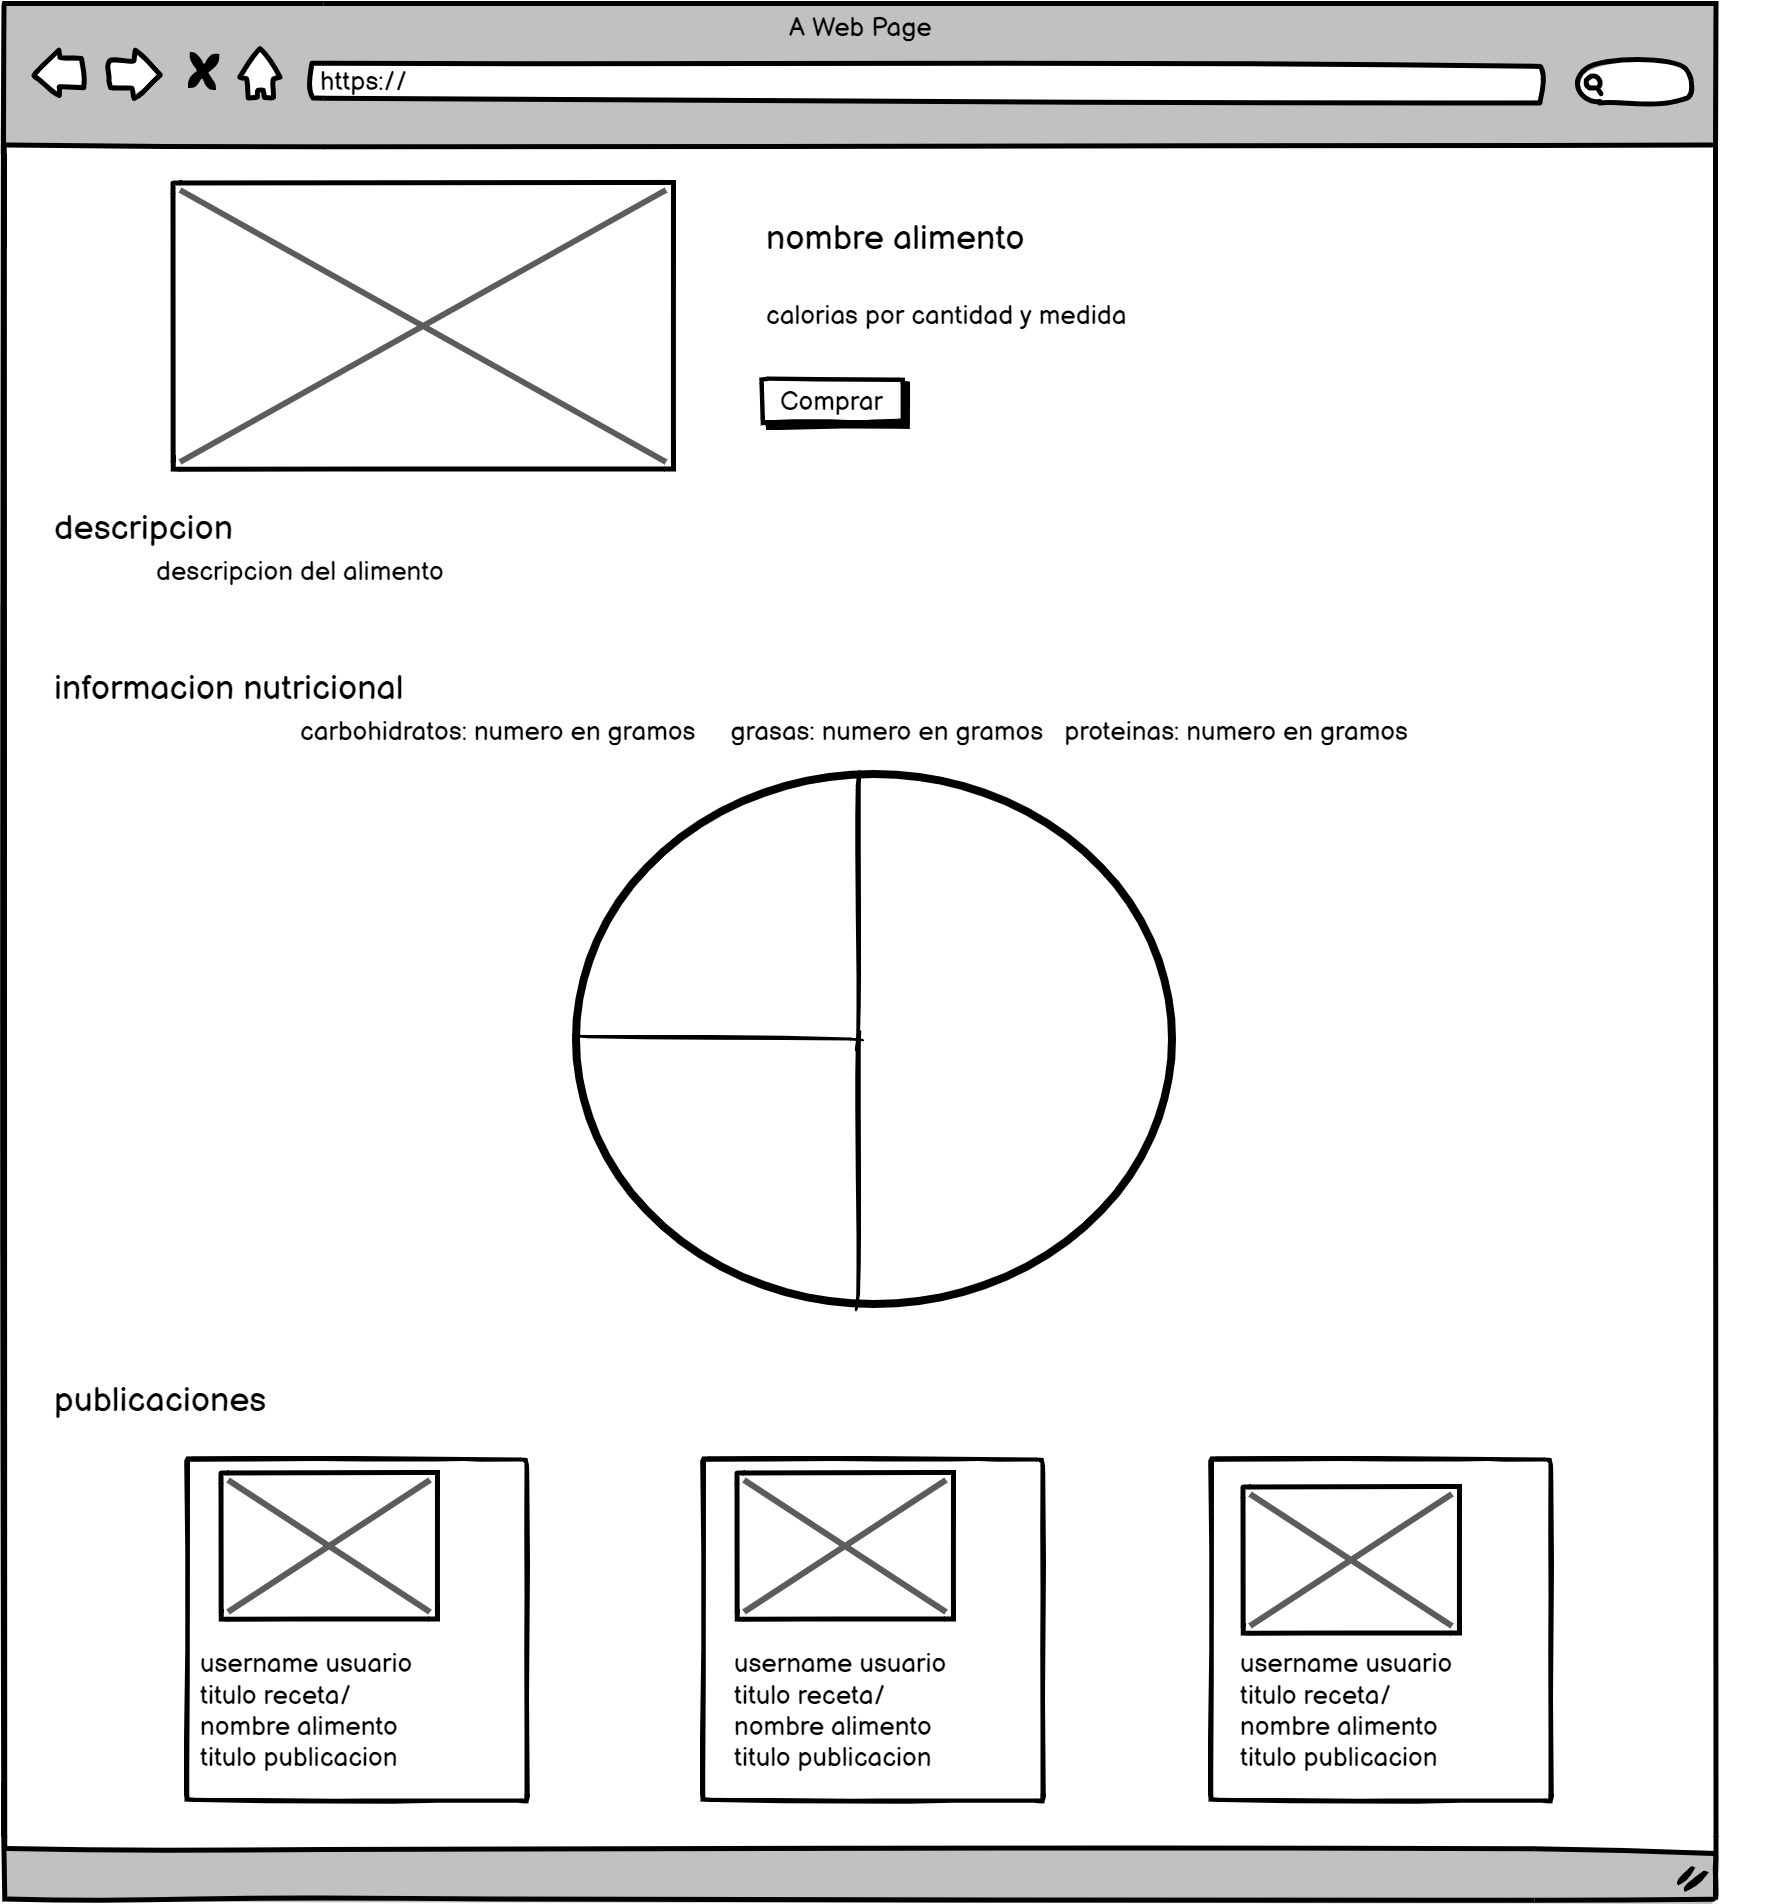
\includegraphics[scale=0.20]{img/detalle-alimento.jpg}
    \caption{Boceto de la interfaz de detalles del alimento.}
    \label{fig:detalle-alimento}
\end{figure}
    
   

      \begin{figure}[H]
    \centering
    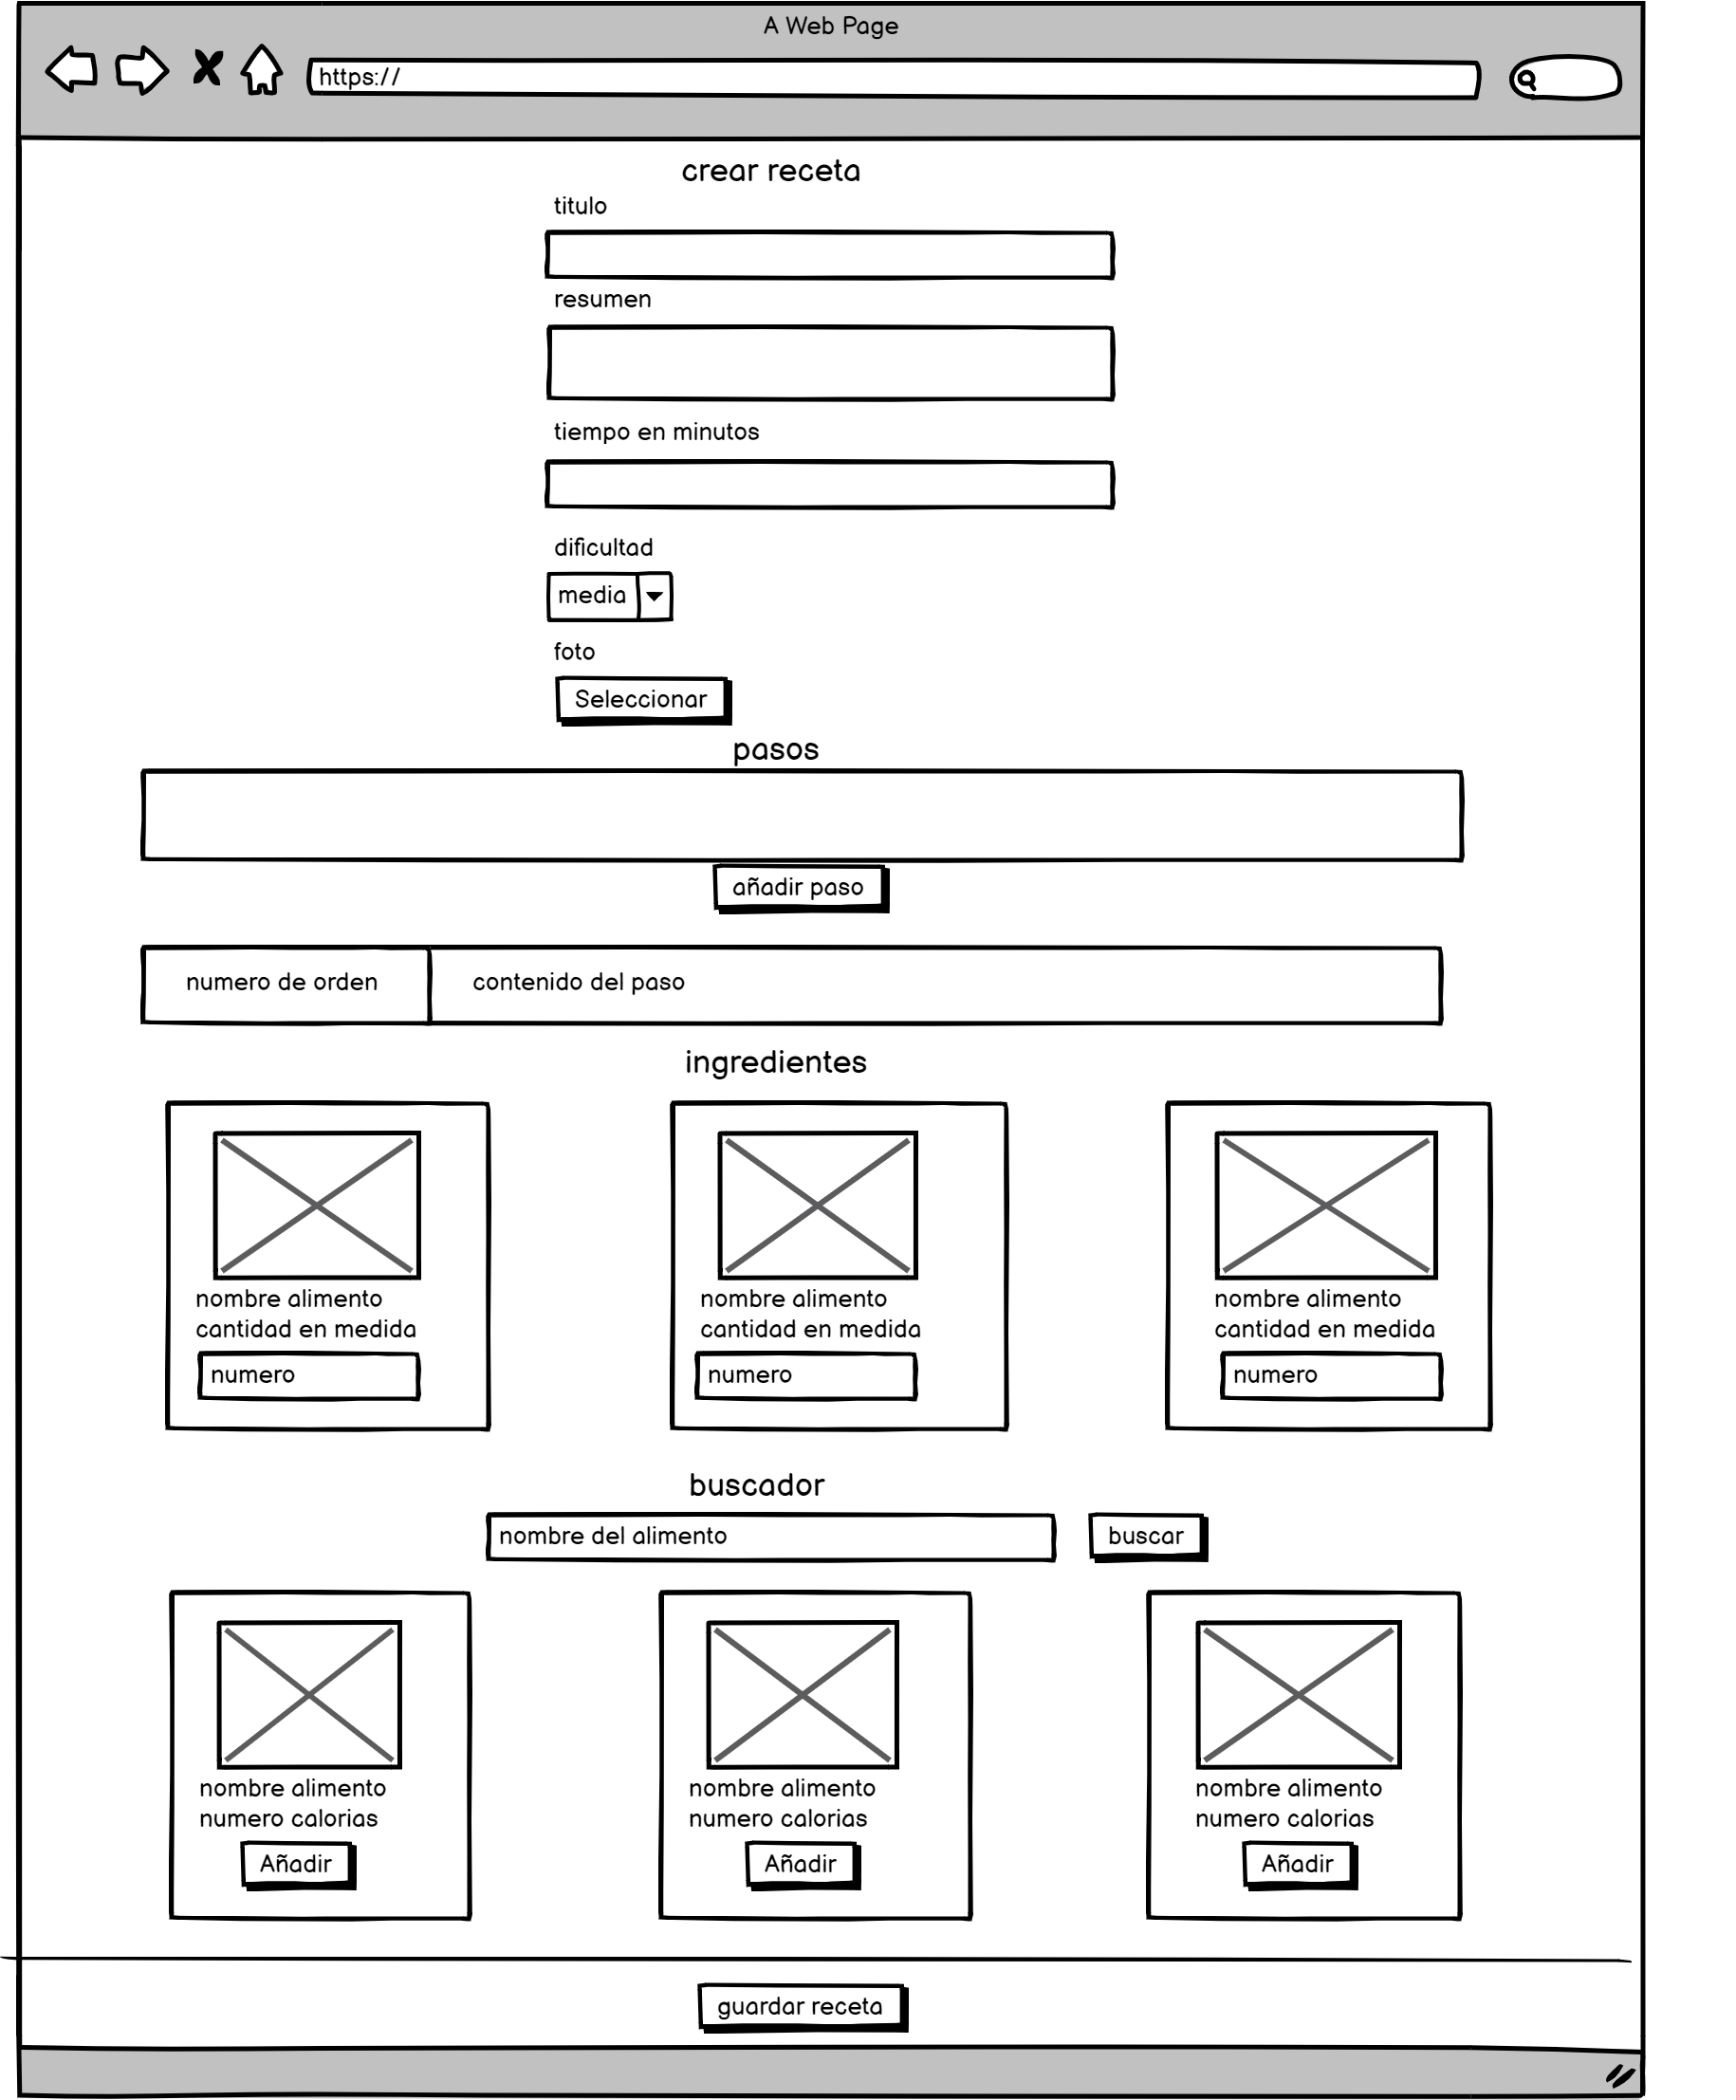
\includegraphics[scale=0.20]{img/crear-receta.jpg}
    \caption{Boceto de la interfaz de crear receta.}
    \label{fig:crear-receta}
\end{figure}
    
  

      \begin{figure}[H]
    \centering
    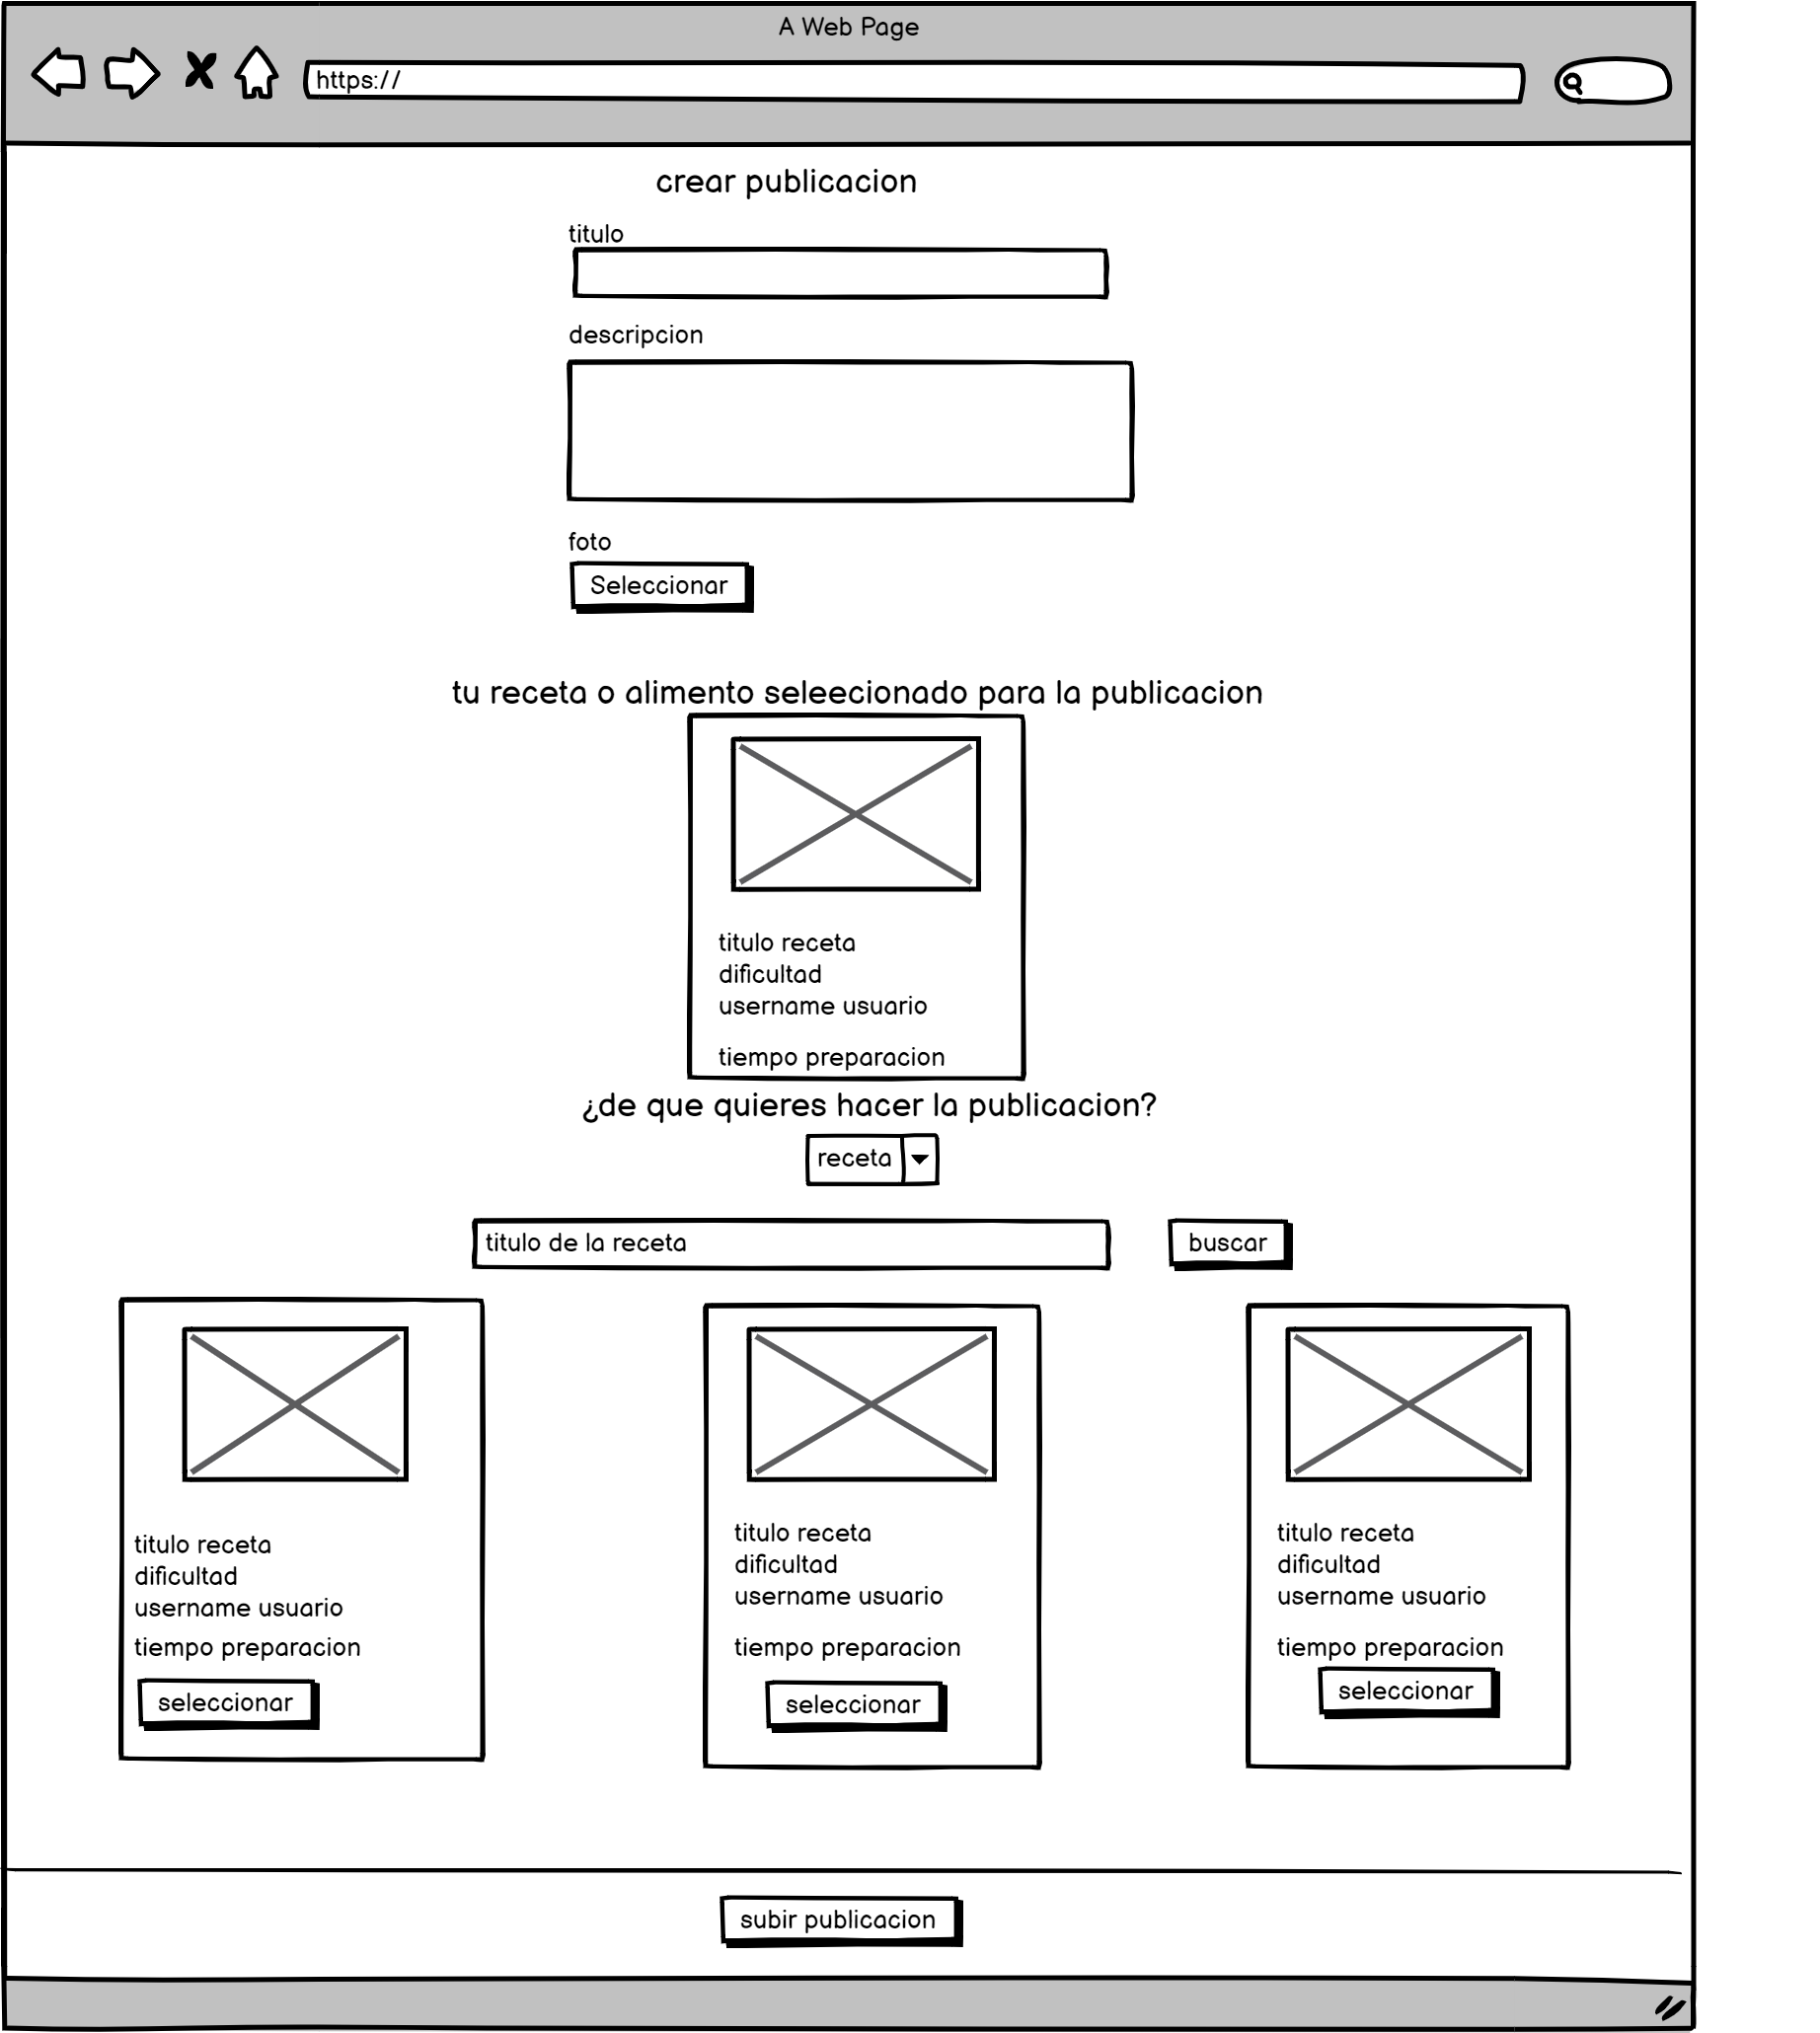
\includegraphics[scale=0.20]{img/crear-publicacion.jpg}
    \caption{Boceto de la interfaz de crear publicación.}
    \label{fig:crear-publicacion}
\end{figure}


   \begin{figure}[H]
    \centering
    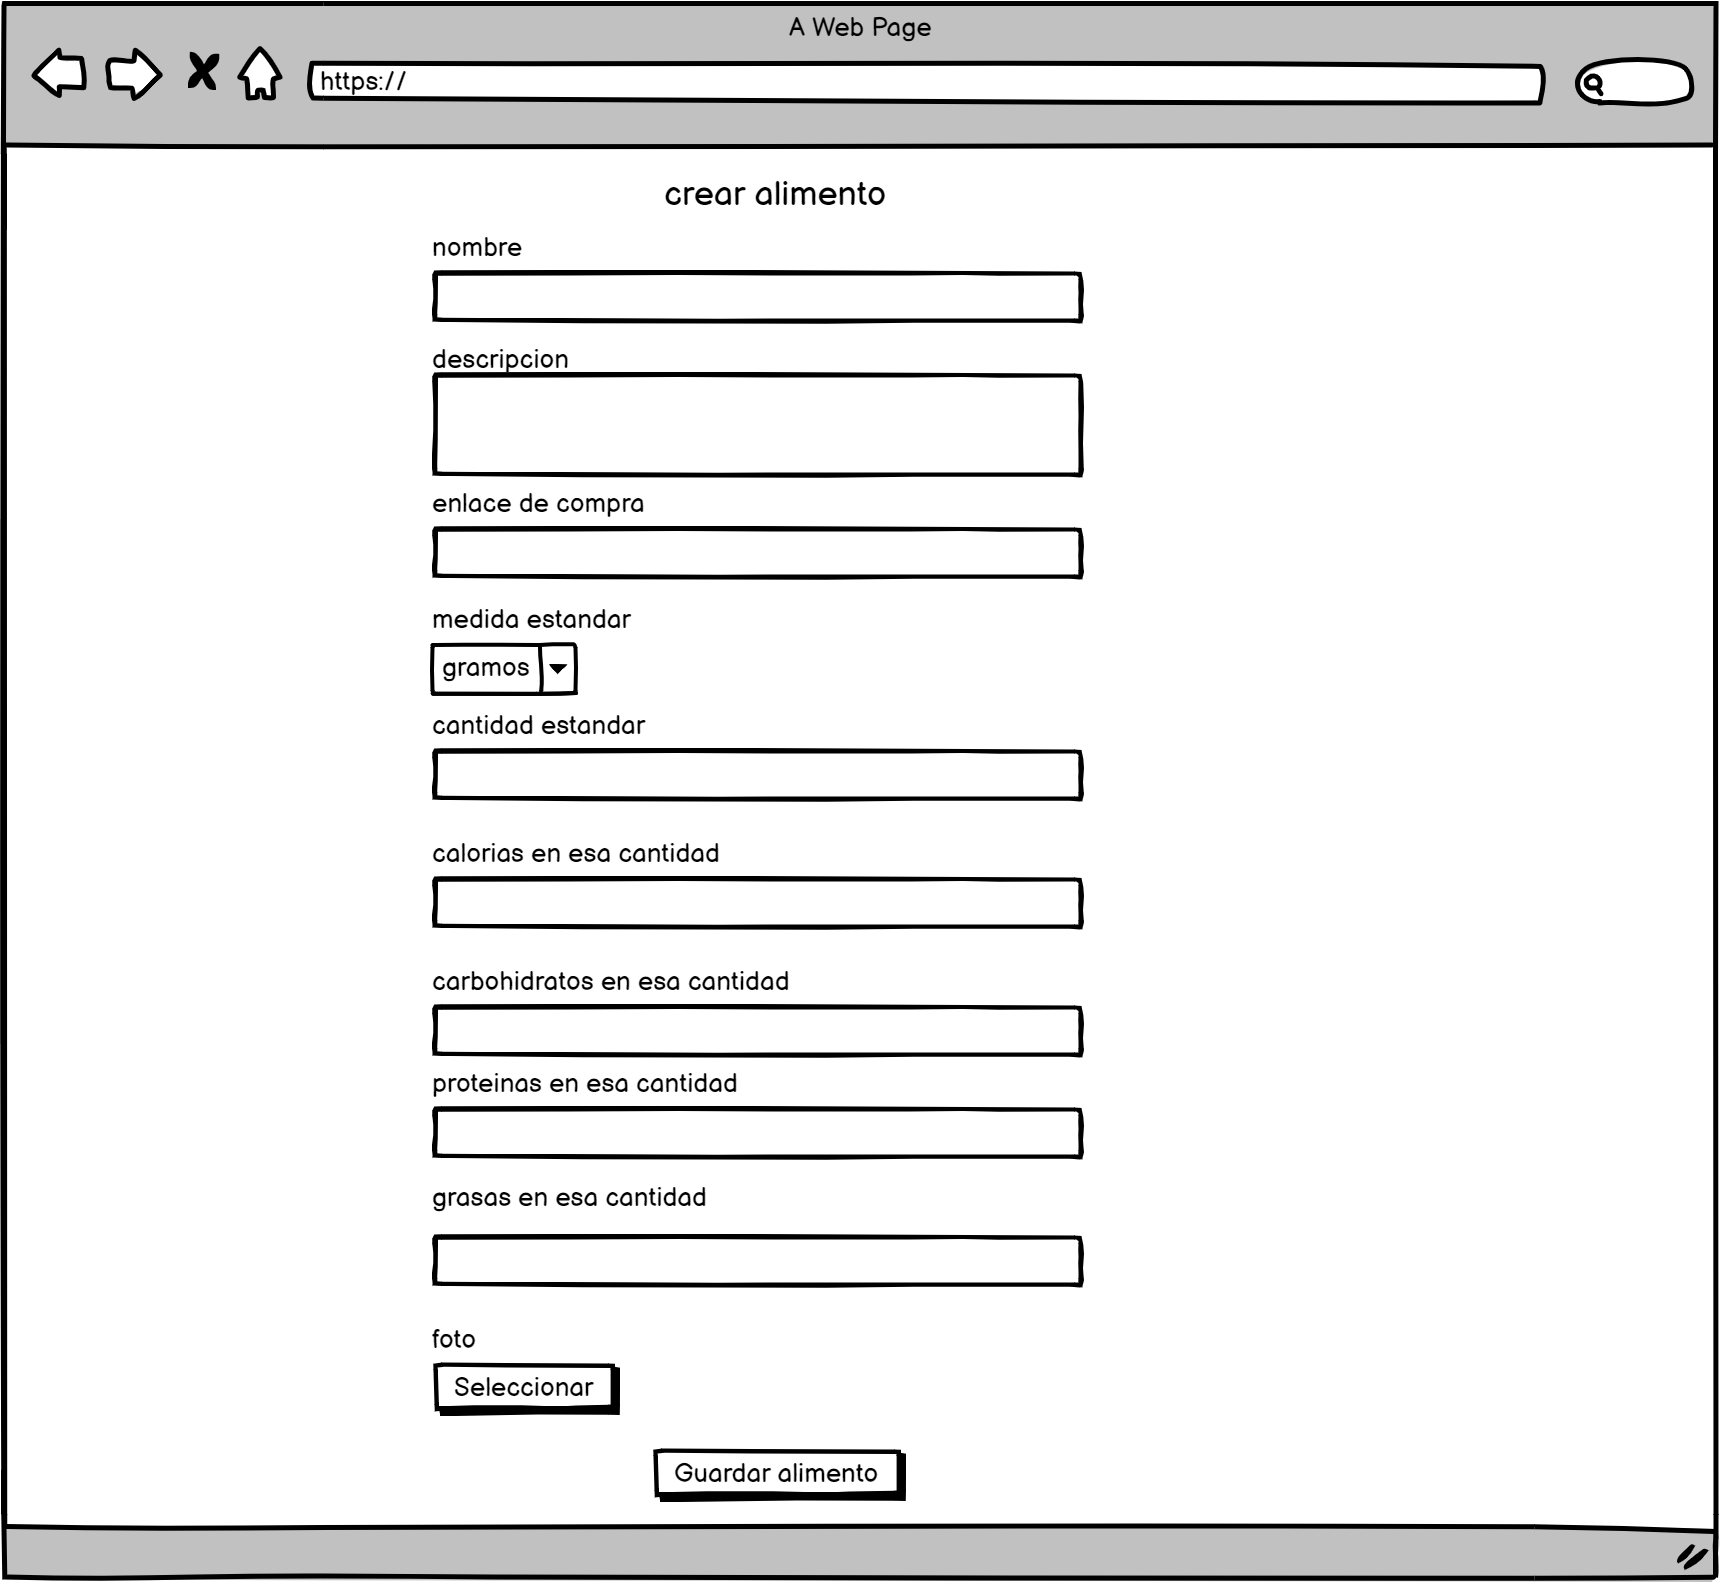
\includegraphics[scale=0.20]{img/crear-alimento.jpg}
    \caption{Boceto de la interfaz de crear alimento.}
    \label{fig:crear-alimento}
\end{figure}
    
 

      \begin{figure}[H]
    \centering
    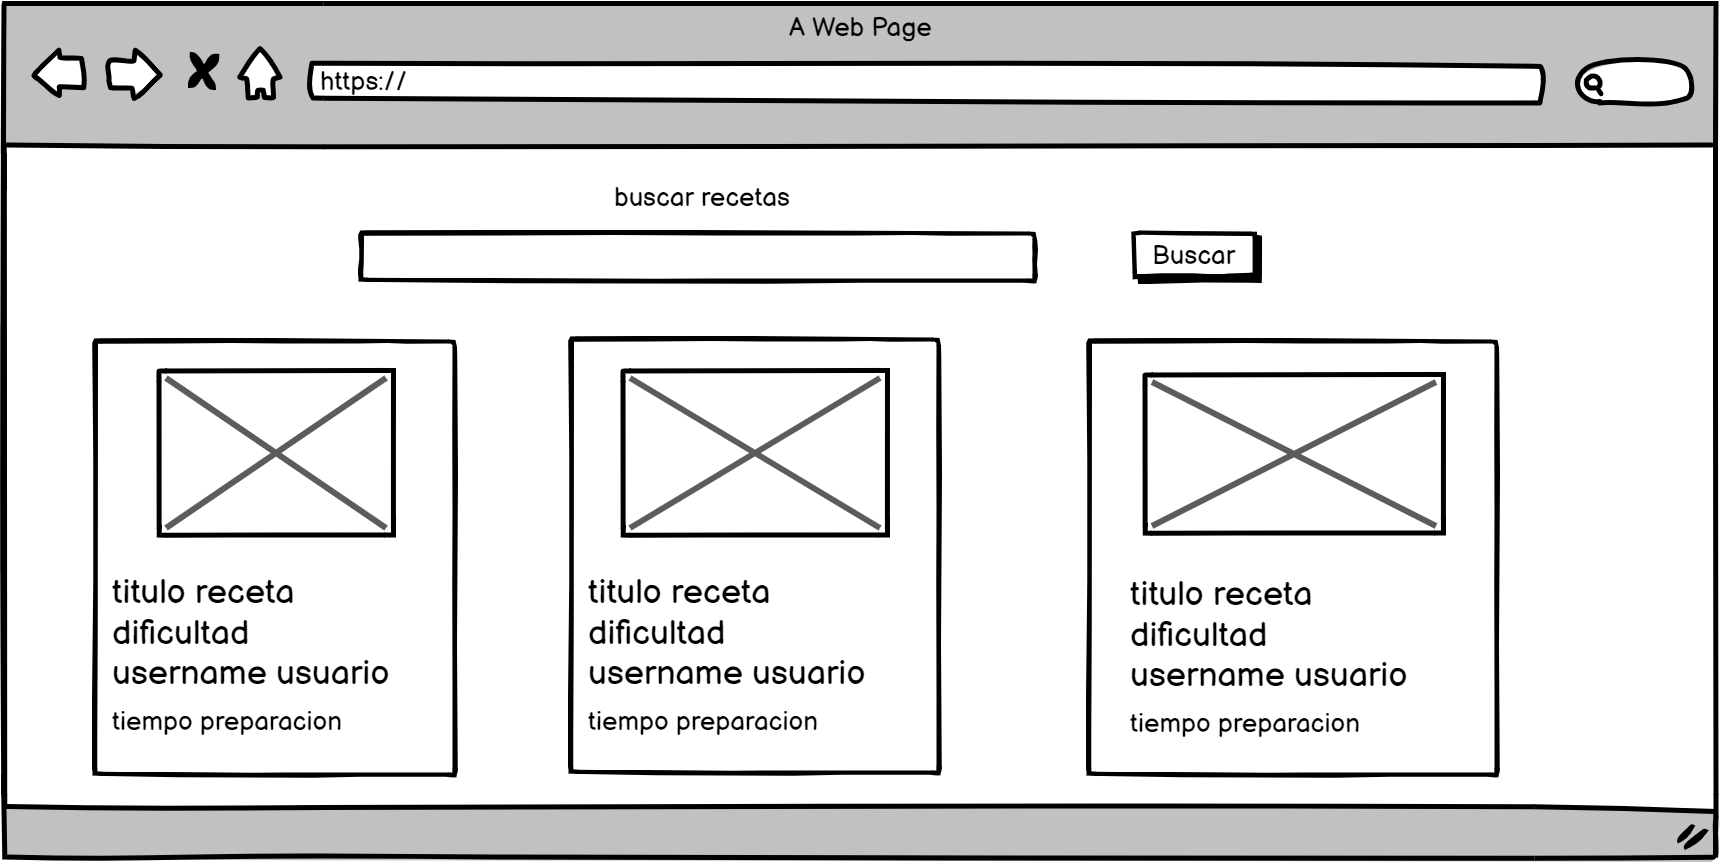
\includegraphics[scale=0.20]{img/buscar-receta.jpg}
    \caption{Boceto de la interfaz de buscador de recetas.}
    \label{fig:buscar-receta}
\end{figure}
    
 
    \begin{figure}[H]
    \centering
    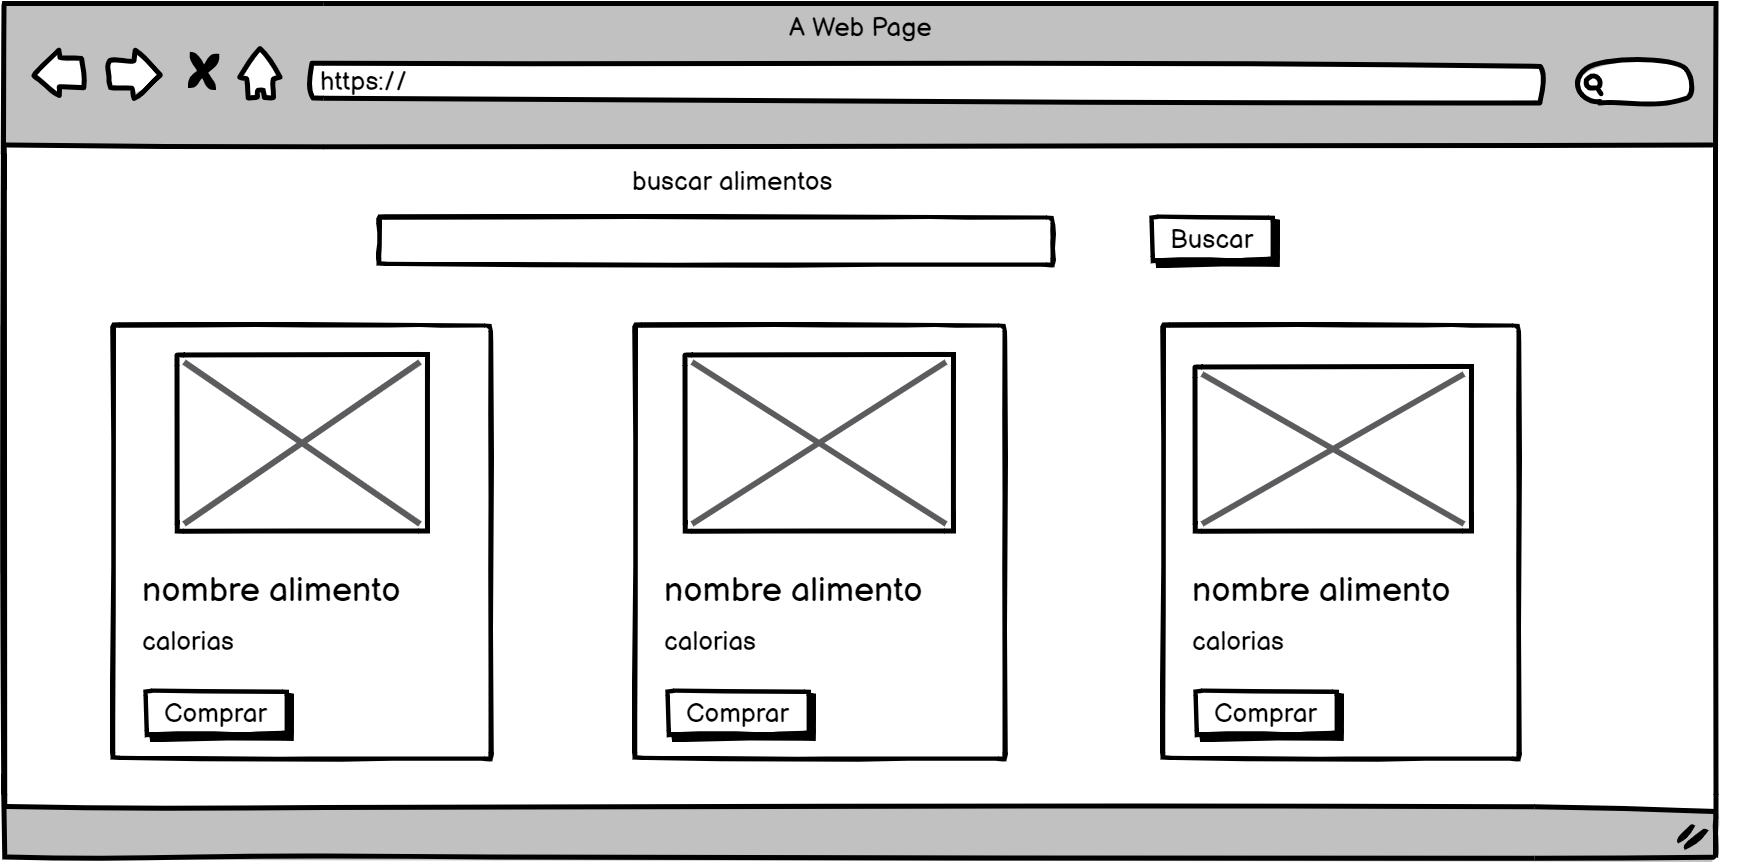
\includegraphics[scale=0.20]{img/buscar-alimento.jpg}
    \caption{Boceto de la interfaz de buscador de alimentos.}
    \label{fig:buscar-alimento}
\end{figure}
    
   

    \begin{figure}[H]
    \centering
    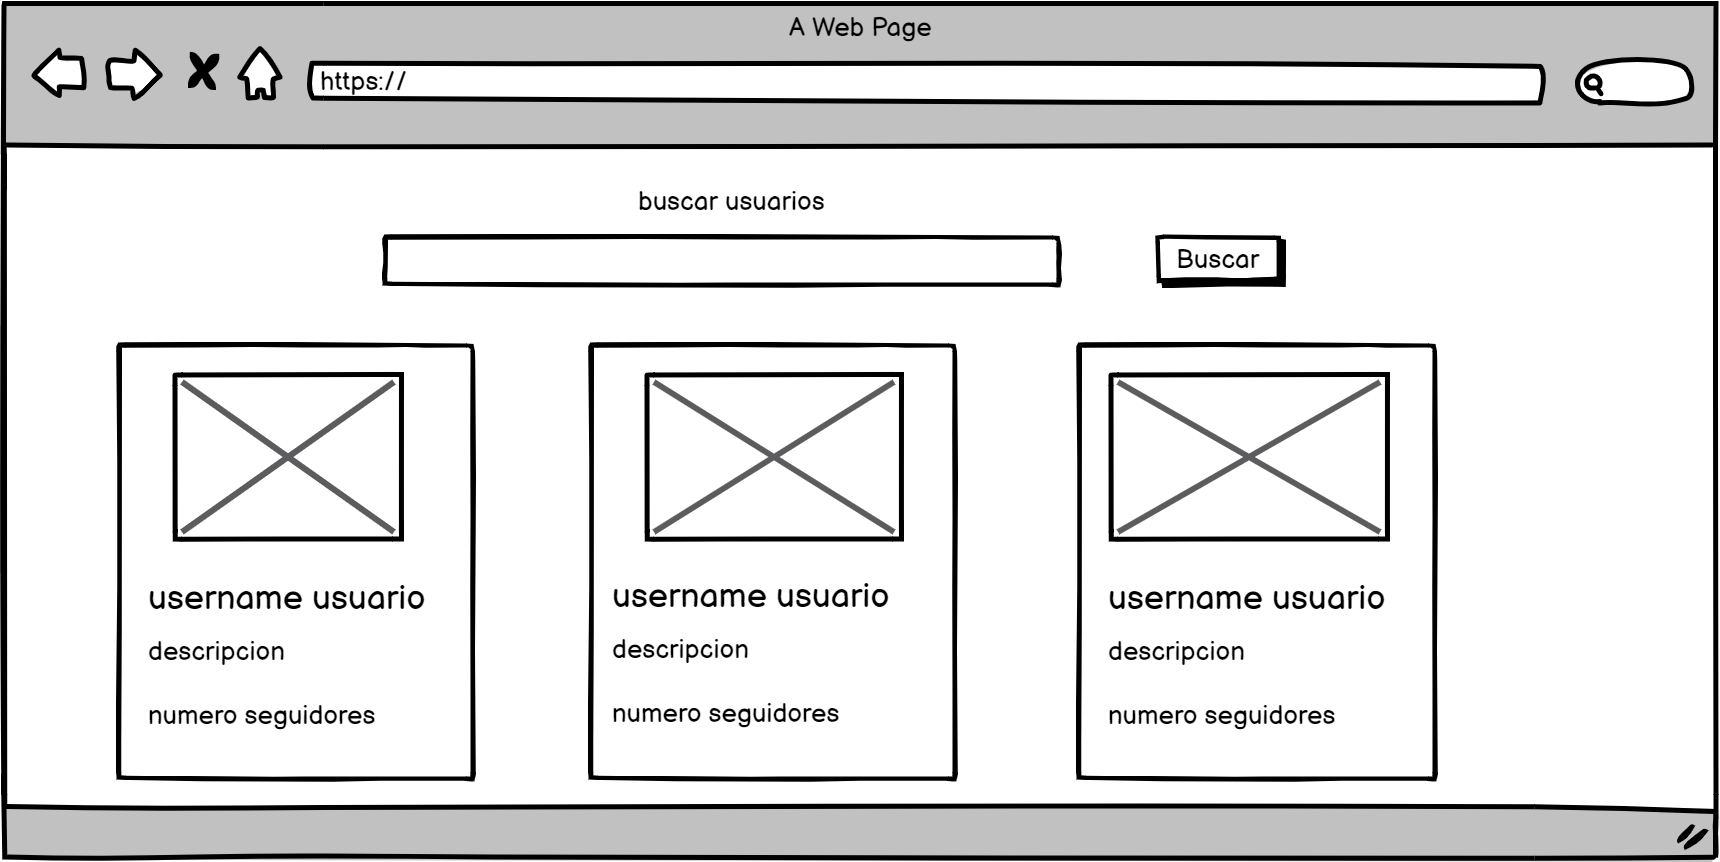
\includegraphics[scale=0.20]{img/buscar-usuario.jpg}
    \caption{Boceto de la interfaz de buscador de usuarios.}
    \label{fig:buscar-usuario}
\end{figure}




 

      \begin{figure}[H]
    \centering
    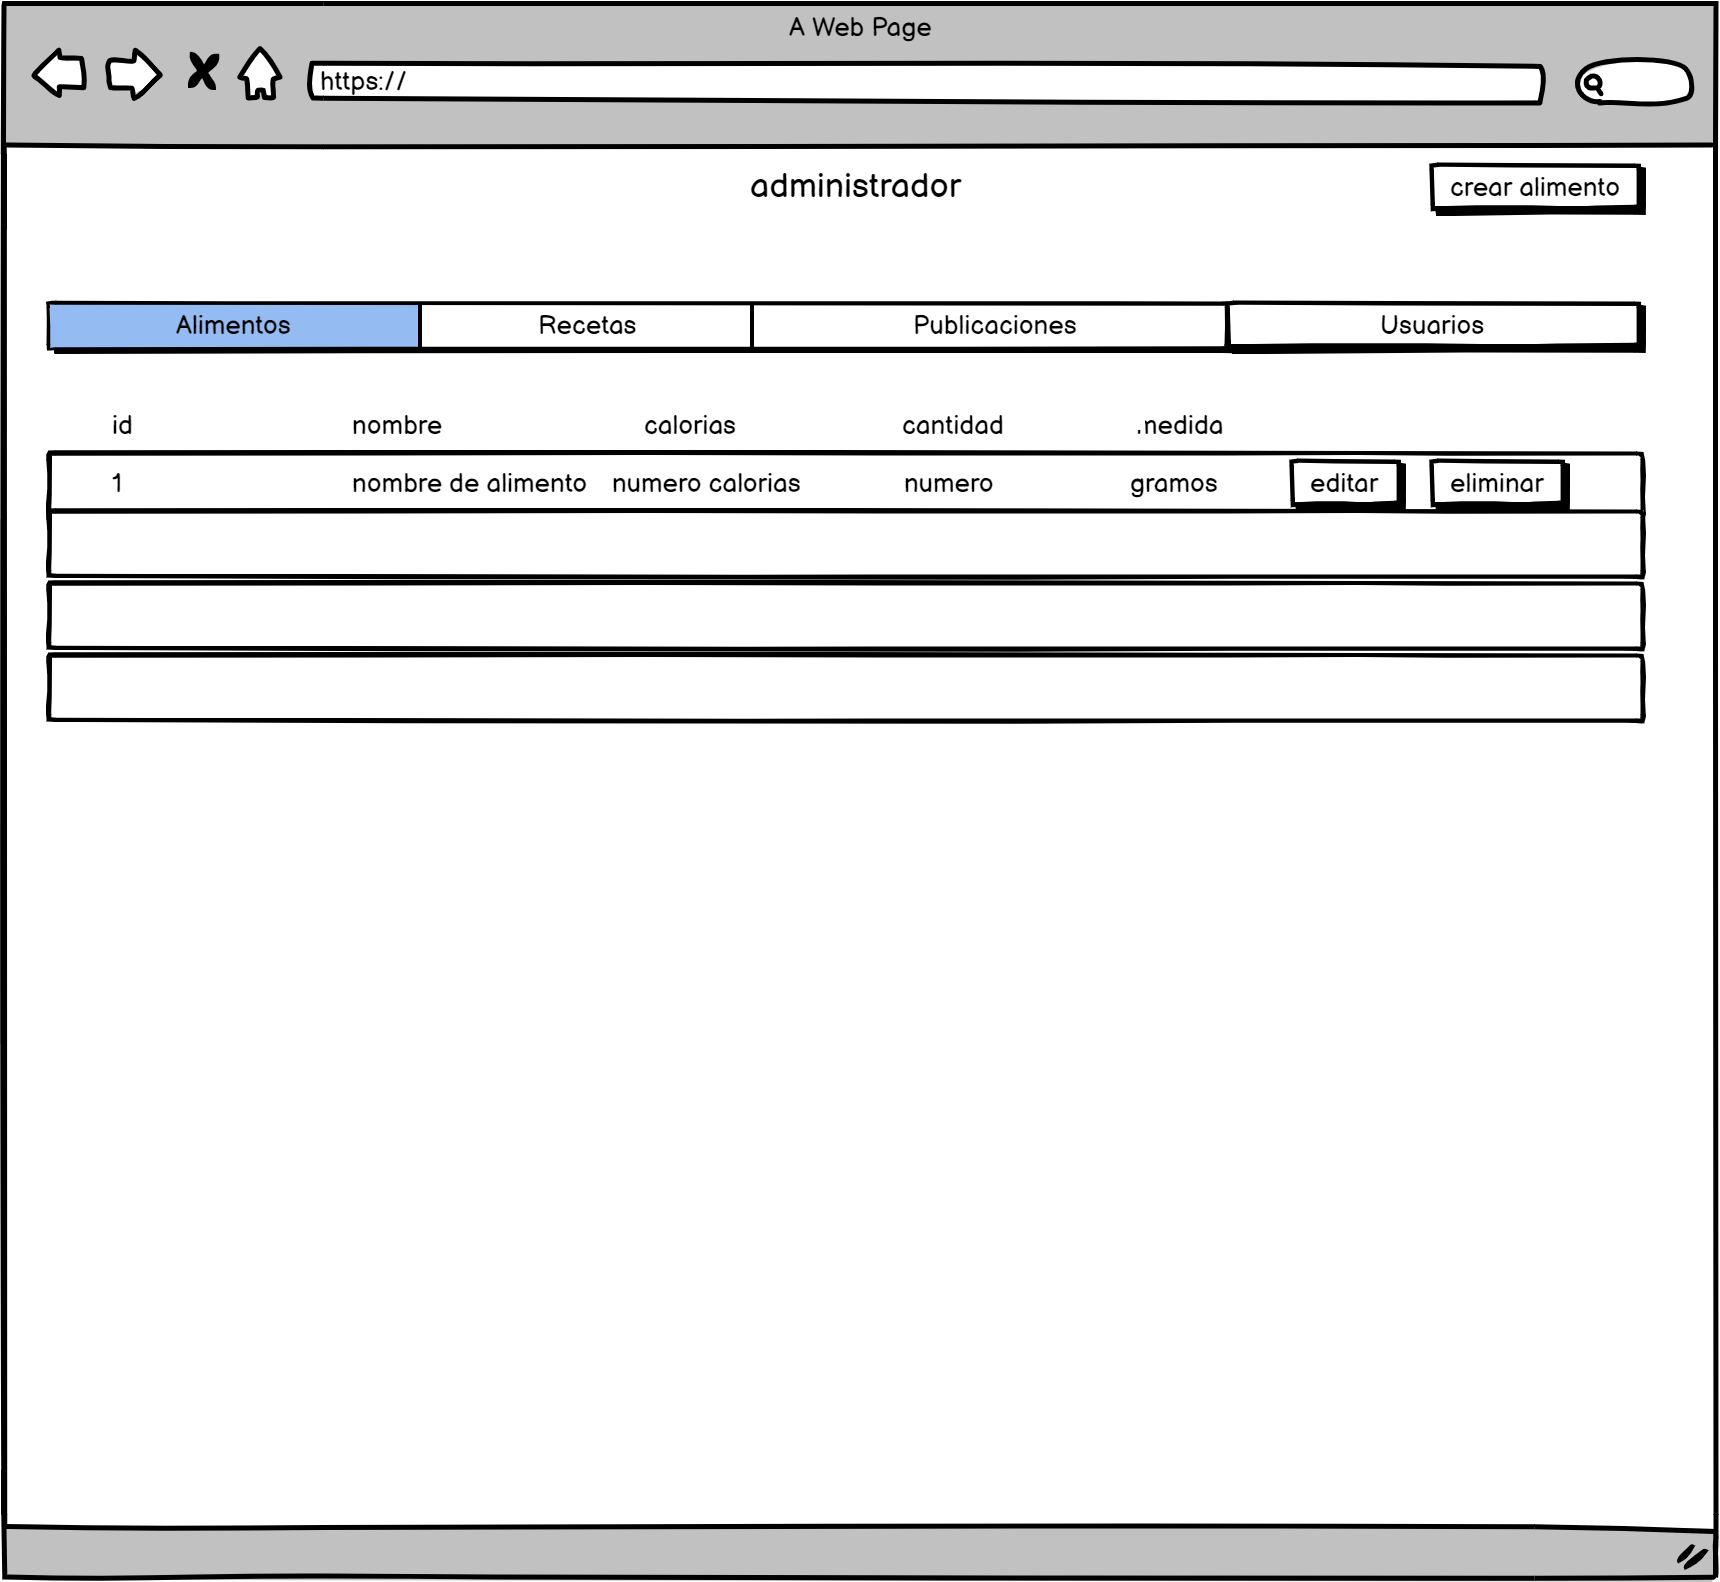
\includegraphics[scale=0.20]{img/vista-admin.jpg}
    \caption{Boceto de la interfaz de vista de Administrador.}
    \label{fig:vista-admin}
\end{figure}



 La selección de los colores para una aplicación Web es importante ya que determinará en gran medida lo que vea el Usuario. Para todo sitio Web cuantos menos colores contenga, será más fácil para el Usuario analizar el sitio Web y de esta forma sea más usable y accesible. Por lo tanto, una buena práctica para el diseño de sitios Web es utilizar tres colores, siendo uno para el fondo, otro para los textos y un color principal que represente la marca personal \cite{colores}. Para este proyecto se han escogido los siguientes colores:

 \begin{itemize}
     \item Color del fondo: blanco: \#FFFFFF
     \item Color del texto: negro: \#000000
     \item Color principal: verde. Se ha escogido el verde como el color principal para la aplicación Web ya que está estrechamente relacionado con la alimentación, en especial con la alimentación saludable. Por lo tanto, se ha escogido el verde claro \#00B347 para las interfaces de la aplicación con la variación del verde oscuro \#00722E para los efectos que haya que realizar cuando el Usuario interactúe con la aplicación Web.
 \end{itemize}

 